\documentclass[11pt,a4paper,oneside,openany]{book}

% ---------------------------------------------------------------------------
% This file, with the chapters it \inputs, is also the source of the
% project's code. build.py pulls every code chunk out of it, rebuilds the
% .nex files from them, runs every program, and checks the result against
% ../*.nex. See build.py.
% ---------------------------------------------------------------------------

\usepackage[margin=2.5cm,top=2.4cm,bottom=2.7cm]{geometry}
\usepackage[T1]{fontenc}
\usepackage[utf8]{inputenc}
\usepackage{amsmath}
\usepackage{amssymb}
\usepackage[sc]{mathpazo}
\usepackage{tgpagella}
\renewcommand{\ttdefault}{txtt}
\usepackage{microtype}
\DisableLigatures[-]{encoding=T1, family=tt*}
\usepackage{xcolor}
\usepackage{listings}
\usepackage[most]{tcolorbox}
\usepackage{tikz}
\usetikzlibrary{arrows.meta,positioning,calc,fit,backgrounds,decorations.pathreplacing}
\usepackage{pgfplots}
\pgfplotsset{compat=1.18}
\usepackage{booktabs}
\usepackage{graphicx}
\usepackage{enumitem}
\usepackage{titlesec}
\usepackage{fancyhdr}
\usepackage[hidelinks]{hyperref}

\setlength{\parindent}{0pt}
\setlength{\parskip}{0.55em}
\linespread{1.06}

\definecolor{accent}{HTML}{1F5F8B}
\definecolor{codebg}{HTML}{F6F8FA}
\definecolor{codeframe}{HTML}{C9D3DD}
\definecolor{titlebg}{HTML}{E4ECF3}
\definecolor{trybg}{HTML}{F3F8EE}
\definecolor{tryframe}{HTML}{B9D3A3}
\definecolor{trytitle}{HTML}{E2EED8}
\definecolor{outbg}{HTML}{2B2F36}
\definecolor{outfg}{HTML}{E8EAED}
\definecolor{kw}{HTML}{0B4F8A}
\definecolor{ty}{HTML}{7A3E9D}
\definecolor{cm}{HTML}{6A737D}
\definecolor{st}{HTML}{22863A}
\definecolor{mathbg}{HTML}{FBF6EA}
\definecolor{mathframe}{HTML}{E2CF9E}

\titleformat{\chapter}[display]
  {\normalfont\color{accent}}
  {\large\scshape \chaptertitlename\ \thechapter}
  {0.2em}
  {\LARGE\bfseries}
\titlespacing*{\chapter}{0pt}{-10pt}{22pt}
\titleformat{\section}{\normalfont\large\bfseries\color{accent}}{\thesection}{0.8em}{}
\titleformat{\subsection}{\normalfont\normalsize\bfseries}{}{0em}{}

\pagestyle{fancy}
\fancyhf{}
\fancyhead[R]{\small\thepage}
\fancyhead[L]{\small\scshape\leftmark}
\renewcommand{\chaptermark}[1]{\markboth{#1}{}}
\renewcommand{\headrulewidth}{0.3pt}
\fancypagestyle{plain}{\fancyhf{}\fancyfoot[C]{\small\thepage}\renewcommand{\headrulewidth}{0pt}}

\lstdefinelanguage{Nex}{
  morekeywords={class,feature,inherit,end,do,if,then,else,elseif,when,from,
    until,invariant,variant,require,ensure,let,as,and,or,not,fn,deferred,
    convert,to,old,create,private,note,with,import,intern,function,raise,
    rescue,retry,assert,repeat,across,case,of,declare,once,match,this,super,
    enum,union,alias,elseif,until,spawn},
  morekeywords=[2]{Integer,Real,Boolean,String,Char,Array,Map,Set,Any,
    Function,Console,Process,Task,Path,Json,Json_Value,Regex,Http_Client,
    Http_Response,Http_Server},
  morekeywords=[3]{true,false,nil,result,exception},
  sensitive=true,
  morecomment=[l]{--},
  morestring=[b]",
}
\lstdefinestyle{nex}{
  language=Nex,
  basicstyle=\ttfamily\footnotesize,
  breaklines=true,
  breakindent=2em,
  postbreak=\mbox{\textcolor{cm}{$\hookrightarrow$}\space},
  keywordstyle=\color{kw}\bfseries,
  keywordstyle=[2]\color{ty},
  keywordstyle=[3]\color{kw},
  commentstyle=\color{cm}\itshape,
  stringstyle=\color{st},
  columns=fullflexible,
  keepspaces=true,
  showstringspaces=false,
  upquote=true,
  extendedchars=true,
  literate={·}{{$\cdot$}}1,
}
\lstdefinestyle{out}{
  language={},
  basicstyle=\ttfamily\footnotesize\color{outfg},
  columns=fullflexible,
  breaklines=true,
  breakindent=2em,
  keepspaces=true,
  extendedchars=true,
}
\lstdefinestyle{shell}{
  language={},
  basicstyle=\ttfamily\footnotesize,
  columns=fullflexible,
  keepspaces=true,
}
\lstset{style=nex}

\tcbset{
  codebox/.style={enhanced, breakable, colback=codebg, colframe=codeframe,
    boxrule=0.5pt, arc=2pt, left=5pt, right=5pt, top=3pt, bottom=3pt,
    colbacktitle=titlebg, coltitle=black, fonttitle=\small,
    toptitle=1.5pt, bottomtitle=1.5pt, before skip=8pt, after skip=8pt},
  trybox/.style={codebox, colback=trybg, colframe=tryframe, colbacktitle=trytitle},
  outbox/.style={enhanced, breakable, colback=outbg, colframe=outbg, arc=2pt,
    boxrule=0pt, left=6pt, right=6pt, top=4pt, bottom=4pt,
    before skip=6pt, after skip=10pt},
}

% The code chunks. The arguments are read by build.py too, so they must
% not contain braces.
%   newfile{file}                    start a new file
%   append{file}                     add at the end of a file
%   addbefore{file}{where}{marker}   add before the line(s) `marker`
%                                    ("|" separates lines); `where` is shown
%   tightaddbefore{...}              the same, without a blank line after
%   continued{file}                  add right after the previous chunk
%   tryit{file}                      a throwaway script to run now
\newtcblisting{newfile}[1]{codebox, listing only, listing options={style=nex},
  title={\textbf{New file}\enspace\texttt{\detokenize{#1}}}}
\newtcblisting{append}[1]{codebox, listing only, listing options={style=nex},
  title={\texttt{\detokenize{#1}}\enspace\textendash\enspace add at the end}}
\newtcblisting{addbefore}[3]{codebox, listing only, listing options={style=nex},
  title={\texttt{\detokenize{#1}}\enspace\textendash\enspace add \detokenize{#2}}}
\newtcblisting{tightaddbefore}[3]{codebox, listing only, listing options={style=nex},
  title={\texttt{\detokenize{#1}}\enspace\textendash\enspace add \detokenize{#2}}}
\newtcblisting{continued}[1]{codebox, listing only, listing options={style=nex},
  title={\texttt{\detokenize{#1}}\enspace\textendash\enspace continued}}
\newtcblisting{tryit}[1]{trybox, listing only, listing options={style=nex},
  title={\textbf{Try it}\enspace\texttt{\detokenize{#1}}}}
\newtcblisting{shell}{codebox, listing only, listing options={style=shell}}
\newtcblisting{textout}{outbox, listing only, listing options={style=out}}

% The output of the try-it script just shown (written by build.py).
\newcommand{\tryoutput}[1]{%
  \begin{tcolorbox}[outbox]
  {\ttfamily\footnotesize\color{outfg}\$ nex \detokenize{#1}.nex}\par\vspace{2pt}
  \lstinputlisting[style=out]{build/out/#1.txt}
  \end{tcolorbox}}
% Run a program at this point of the tutorial and show its output.
\newcommand{\runoutput}[2]{%
  \begin{tcolorbox}[outbox]
  {\ttfamily\footnotesize\color{outfg}\$ nex \detokenize{#1}}\par\vspace{2pt}
  \lstinputlisting[style=out]{build/out/#2.txt}
  \end{tcolorbox}}

% The output saved by a \runoutput later in the tutorial, shown early.
\newcommand{\laterout}[2]{%
  \begin{tcolorbox}[outbox]
  {\ttfamily\footnotesize\color{outfg}\$ nex \detokenize{#1}}\par\vspace{2pt}
  \lstinputlisting[style=out]{build/out/#2.txt}
  \end{tcolorbox}}

\newtcolorbox{mathbox}[1][]{enhanced, breakable, colback=mathbg,
  colframe=mathframe, boxrule=0.5pt, arc=2pt, left=8pt, right=8pt,
  top=4pt, bottom=4pt, fonttitle=\bfseries\small, coltitle=black,
  colbacktitle=mathframe!45, title={#1}, before skip=8pt, after skip=8pt}
\newtcolorbox{aside}{enhanced, breakable, colback=white, colframe=accent,
  boxrule=0pt, leftrule=2.5pt, arc=0pt, left=8pt, right=4pt, top=2pt,
  bottom=2pt, before skip=8pt, after skip=8pt}

\newcommand{\code}[1]{\texttt{\detokenize{#1}}}

% Code from elsewhere, shown but not part of the project (build.py ignores it).
\newtcblisting{excerpt}[1]{codebox, listing only, listing options={style=nex},
  title={\texttt{\detokenize{#1}}\enspace\textendash\enspace an excerpt}}
% A JSON message, as the API sends and receives it.
\newtcblisting{json}{codebox, listing only, listing options={style=shell}}

\hypersetup{pdftitle={A Coding Agent in Nex},
  pdfsubject={How a coding agent works, built from scratch, step by step}}

\begin{document}

% ---------------------------------------------------------------------------
\begin{titlepage}
\centering
\vspace*{3.0cm}
{\color{accent}\rule{\linewidth}{0.8pt}}\par\vspace{0.9cm}
{\Huge\bfseries A Coding Agent\par}
\vspace{0.35cm}
{\LARGE in Nex\par}
\vspace{0.9cm}
{\large How a program that reads, edits and tests code\\[2pt]
  with a language model works, built from scratch\par}
\vspace{0.9cm}
{\color{accent}\rule{\linewidth}{0.8pt}}\par
\vspace{1.6cm}

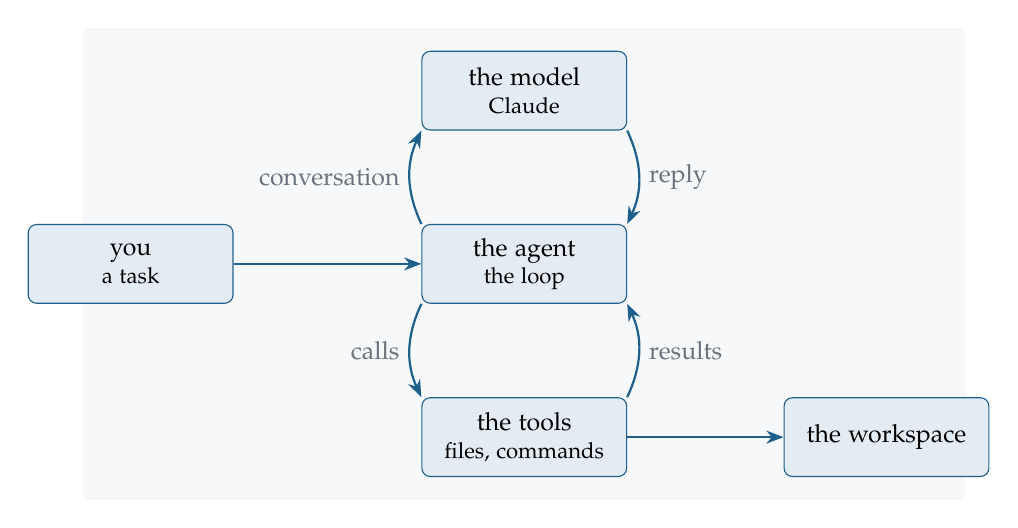
\begin{tikzpicture}[x=1cm,y=1cm, font=\small,
    box/.style={draw=accent, fill=titlebg, rounded corners=3pt, minimum width=2.6cm,
      minimum height=1.0cm, align=center},
    arr/.style={-{Stealth[length=2.2mm]}, accent, line width=0.8pt}]
  \fill[codebg] (-0.6,-2.0) rectangle (10.6,4.0);
  \node[box] (you) at (0,1) {you\\[-1pt]\footnotesize a task};
  \node[box] (agent) at (5,1) {the agent\\[-1pt]\footnotesize the loop};
  \node[box] (model) at (5,3.2) {the model\\[-1pt]\footnotesize Claude};
  \node[box] (tools) at (5,-1.2) {the tools\\[-1pt]\footnotesize files, commands};
  \node[box] (ws) at (9.6,-1.2) {the workspace};
  \draw[arr] (you) -- (agent);
  \draw[arr] (agent.north west) to[bend left=25] node[left, text=cm] {conversation} (model.south west);
  \draw[arr] (model.south east) to[bend left=25] node[right, text=cm] {reply} (agent.north east);
  \draw[arr] (agent.south west) to[bend right=25] node[left, text=cm] {calls} (tools.north west);
  \draw[arr] (tools.north east) to[bend right=25] node[right, text=cm] {results} (agent.south east);
  \draw[arr] (tools) -- (ws);
\end{tikzpicture}

\vfill
{\large A step-by-step tutorial\par}
\vspace{0.3cm}
{\normalsize Every line of code, nothing hidden\par}
\vspace{1.5cm}
\end{titlepage}

\frontmatter
\tableofcontents
\mainmatter

% ===========================================================================
\chapter{What we are going to build}

A \emph{coding agent} is a program you give a task in plain words, such as
``some of the checks fail; find out why and fix it'', and that then works
on a project by itself. It looks at the files, runs the tests, reads the
code that matters, changes it, runs the tests again, and tells you what it
did. The thinking is done by a large language model: in this tutorial,
Claude. The agent is the program around the model, and that program is
what we are going to write, in Nex, from scratch.

Here is the finished agent at work on a small project, a lending library
whose fines come out wrong. Everything the agent does is printed as it
happens: what the model says, each tool it asks for (indented), and the
first line of what each tool gave back.

\laterout{code.nex --replay sessions/fix_late_fines.json --yes}{replay}

The model never touches the project. All it can do is write text. What
makes it an agent is that some of that text is a request to use a tool:
``run \code{nex checks.nex}'', ``show me \code{loans.nex}'', ``replace
these two lines with those''. Our program carries out each request, and
sends back what happened. Then the model writes some more. The whole agent
is this loop:

\begin{shell}
conversation := [the task]
repeat
    reply := the model's answer to the conversation
    add the reply to the conversation
    if the reply asks for tools then
        run them, and add what they gave back to the conversation
    else
        the task is done
\end{shell}

That is the whole idea, and Chapter~\ref{ch:loop} writes it in about forty
lines. Most of the work, and most of this tutorial, goes into what is
around the loop: tools that are safe to hand to a model and give it useful
answers, edits that fail loudly instead of quietly doing the wrong thing,
a workspace the agent cannot reach outside of, permission before anything
changes, limits, recovery from errors, and keeping the conversation from
growing for ever.

\begin{aside}
\textbf{Where the safety lives.} The model only ever \emph{asks}. Whether a
file is read, an edit is made or a command is run is decided by our
program, every time. So the rules that keep an agent safe (which folder it
may touch, what needs your permission) are ordinary code, with ordinary
contracts, that we write and check like any other.
\end{aside}

\section{How this tutorial works}

We build the agent file by file, in the order you would write it. Every
line of every file appears in the text, in boxes. A box titled \emph{New
file} starts a file. Other boxes add to a file you already have: \emph{add at the end},
\emph{add before} a given line, or \emph{continued} (right after the box
before). Follow them and you end up with the project in
\code{examples/coding_agent} of the Nex distribution, exactly: this
tutorial is built from the same source as the code, and the build checks
that the two match.

Green boxes are \emph{try-it} scripts: small throwaway programs that show
what the code so far does. The dark boxes under them are what they print,
copied from a real run, as is every output in this tutorial.

You need no language model to follow along. Until Chapter~\ref{ch:claude},
the model is played by a script we write ourselves, which lets us test
every part of the agent with replies we choose. After that, a recorded
session plays the model's part, so the outputs in this tutorial are the
same every time it is built. To have Claude itself do the work, you need
an API key, and Chapter~\ref{ch:program} shows how to use it.

\section{What you need}

\begin{itemize}
\item Nex 0.6.5 or later, with \code{nex} on your \code{PATH}. The agent
  runs \code{nex} itself, to run the checks of the project it works on.
\item \code{bash}, for the commands the agent runs. Linux and macOS have
  it.
\item Optionally, a Claude API key from \code{console.anthropic.com}, to
  run the agent for real.
\end{itemize}

You do not need to know anything about language models. You should know
some Nex, or another language in the same family; anything new is
explained when it first comes up, and Appendix~\ref{app:api} puts the API
on one page.

\section{The plan}

\begin{center}
\begin{tabular}{@{}ll@{}}
\toprule
Chapter & What we add \\
\midrule
\ref{ch:setup}. Setting up & the project folder; text helpers \\
\ref{ch:conversation}. A conversation as data & messages, tool calls, replies \\
\ref{ch:model}. A pretend model & the \code{Model} class, and a model played by a script \\
\ref{ch:workspace}. A place to work & a workspace the agent can't reach outside of \\
\ref{ch:tools}. Giving the model hands & tools: listing and reading files \\
\ref{ch:loop}. The agent loop & the agent itself \\
\ref{ch:search}. Finding things & searching the code \\
\ref{ch:editing}. Changing things safely & editing and writing files \\
\ref{ch:commands}. Running commands & running checks, with a time limit \\
\ref{ch:permission}. Asking first & permission before anything changes \\
\ref{ch:claude}. Talking to Claude & the Messages API, over HTTP \\
\ref{ch:replay}. Record and replay & sessions you can play back \\
\ref{ch:program}. The program & \code{code.nex}, the agent on the command line \\
\ref{ch:long}. Long conversations & counting tokens; summing up and starting afresh \\
\ref{ch:checks}. Trust, but verify & executable checks for all of it \\
\ref{ch:next}. Where to go next & streaming, sub-agents, undo, \ldots \\
\bottomrule
\end{tabular}
\end{center}

% ===========================================================================
\chapter{Setting up}\label{ch:setup}

Make a folder for the project and go into it. Every file in this tutorial
goes in this one folder.

\begin{shell}
mkdir agent
cd agent
\end{shell}

Copy two folders into it from \code{examples/coding_agent} of the Nex
distribution:

\begin{itemize}
\item \code{sample_project}, the project the agent will work on: a small
  lending library, with a bug;
\item \code{sessions}, which holds a recorded session, for
  Chapter~\ref{ch:replay}.
\end{itemize}

\section{The sample project}

\code{sample_project} has three Nex files and a \code{README.md}. A
\code{Loan} is a book lent to someone on some day (days are numbered from
the day the library opened), and is due back 14 days later:

\begin{excerpt}{sample_project/loans.nex}
  -- The last day the book may be returned without a fine.
  due_on(): Integer do
    result := lent_on + LOAN_DAYS
  end

  -- How many days late a book returned on `day` is: 0 if on time.
  days_late(day: Integer): Integer
  require
    not_before_loan: day >= lent_on
  do
    if day >= due_on() then
      result := day - due_on() + 1
    end
  ensure
    never_negative: result >= 0
  end
\end{excerpt}

A \code{Fine_Policy} charges so many cents for each day late, up to a
maximum. And \code{checks.nex} checks both. Run the checks:

\begin{shell}
cd sample_project
nex checks.nex
\end{shell}

Four of the seven fail. You may already see why, but don't fix it: that is
the agent's job. (If you do fix it, copy the folder again.)

\section{A first file: text helpers}

An agent spends most of its time moving text around: file contents,
command output, the model's replies. The first file holds the small text
utilities the rest of the project uses.

First, a word about printing. Nex's \code{print} shows a string with its
quotes, as \code{"hello"}, which is handy when debugging but not in a
program's output. Every Nex program has a \code{Console} called
\code{console}, ready to use without creating it, and
\code{console.print_line("hello")} prints the text as it is, on a line of
its own. We use it for all our output.

Nex strings have \code{index_of}, which finds the first place a piece of
text occurs. We will often need the next place after some position, to
count occurrences or to split text into lines, so the first helper does
that. It searches the rest of the string, from \code{start} on, and adds
\code{start} back to the position it finds:

\begin{newfile}{helpers.nex}
-- helpers.nex: small text utilities the rest of the agent uses, and
-- finding the user's files.

-- Where `part` first occurs in `text` at or after position `start`, or -1.
function index_from(text, part: String, start: Integer): Integer
require
  part_given: part /= ""
  start_in_range: start >= 0 and start <= text.length
do
  let at: Integer := text.substring(start, text.length).index_of(part)
  result := when at < 0 then -1 else start + at end
ensure
  not_found_or_after: result = -1 or result >= start
end
\end{newfile}

The \code{require} clause is the function's precondition: what must be true
when it is called. Searching for the empty string makes no sense, and a
start outside the string is a mistake by the caller. If a call breaks a
precondition, Nex stops with an error that names the clause, such as
\code{Precondition violation: part_given}, instead of carrying on with
nonsense. The \code{ensure} clause, the postcondition, is what the function
promises in return. We will lean on contracts like these throughout: they
say what each piece of code expects and guarantees, and Nex checks them as
the program runs.

\code{when} \ldots\ \code{then} \ldots\ \code{else} \ldots\ \code{end} is
an \code{if} that gives a value.

Now we can count how many times a piece of text occurs. This will be the
heart of the agent's safe editing in Chapter~\ref{ch:editing}: an edit is
only allowed if the text to replace occurs exactly once.

\begin{append}{helpers.nex}
-- How many times `part` occurs in `text`, not counting overlaps:
-- count_occurrences("banana", "an") is 2.
function count_occurrences(text, part: String): Integer
require
  part_given: part /= ""
do
  let at: Integer := index_from(text, part, 0)
  from until at < 0 do
    result := result + 1
    at := index_from(text, part, at + part.length)
  end
ensure
  never_negative: result >= 0
end

-- `text` with its first `before` replaced by `after`.
function replace_first(text, before, after: String): String
require
  occurs: text.index_of(before) >= 0
do
  let at: Integer := text.index_of(before)
  result := text.substring(0, at) + after + text.substring(at + before.length, text.length)
end
\end{append}

\code{from} \ldots\ \code{until} \ldots\ \code{do} \ldots\ \code{end} is
Nex's loop: it repeats the body until the condition becomes true. An
\code{Integer} \code{result} starts at 0, so \code{count_occurrences} can
add to it straight away.

Why not use the strings' own \code{split} to cut text into lines? Because
it takes a regular expression rather than plain text, and it drops empty
pieces at the end. Files are made of lines, and an agent has to show them
faithfully, blank lines and all, so we write our own:

\begin{append}{helpers.nex}
-- The lines of `text`, without their line breaks. A final line break
-- does not start another line: lines_of("a\nb\n") is ["a", "b"], and
-- lines_of("") is [].
function lines_of(text: String): Array[String] do
  let start: Integer := 0
  from until start >= text.length do
    let stop: Integer := index_from(text, "\n", start)
    if stop < 0 then
      stop := text.length
    end
    result.add(text.substring(start, stop))
    start := stop + 1
  end
end

-- Lines joined back together, each ending in a line break.
function joined_lines(lines: Array[String]): String do
  result := ""
  across lines as line do
    result := result + line + "\n"
  end
end
\end{append}

An \code{Array} \code{result} starts out empty, ready to \code{add} to.
\code{across} \ldots\ \code{as} \ldots\ \code{do} runs its body once for
every element.

When the agent shows the model a file, it numbers the lines, so that the
model can say ``line 32'' and we can see what it means. \code{pad_start}
adds spaces on the left until the number is 5 characters wide:

\begin{append}{helpers.nex}
-- `lines` numbered from `first`, the way read_file shows a file:
--    12  some code
function numbered(lines: Array[String], first: Integer): String do
  result := ""
  let n: Integer := first
  across lines as line do
    result := result + n.to_string.pad_start(" ", 5) + "  " + line + "\n"
    n := n + 1
  end
end
\end{append}

\section{Keeping output short}

A model reads everything we send it, and pays for it, in time and money:
models read text as \emph{tokens}, pieces of a few characters each, and
are priced by the token. A command can print a megabyte. So every tool's
output will be cut down to a sensible size before the model sees it.
Which part to keep? Usually the beginning and the end: the beginning says
what a command was doing, the end how it finished (the error, or the
summary line of a test run). So \code{shortened} drops the middle, and says
how much it dropped:

\begin{append}{helpers.nex}
-- `text` cut down to at most about `limit` characters by dropping the
-- middle. The start and the end of a long output are usually the useful
-- parts: what a command was doing, and how it finished.
function shortened(text: String, limit: Integer): String
require
  sensible_limit: limit >= 100
do
  if text.length <= limit then
    result := text
  else
    let keep: Integer := (limit - 60) / 2
    let cut: Integer := text.length - 2 * keep
    result := text.substring(0, keep)
      + "\n[... " + cut.to_string + " characters cut ...]\n"
      + text.substring(text.length - keep, text.length)
  end
ensure
  short_enough: result.length <= limit
end
\end{append}

The 60 characters left over are room for the note in the middle; the
postcondition checks that it fits.

The next helpers are for what the agent prints for you: a one-line preview
of a long text, counts like ``3 lines'' and ``2 replies'', and indenting:

\begin{append}{helpers.nex}
-- The first line of `text`, cut to `limit` characters: a one-line preview.
function preview(text: String, limit: Integer): String
require
  sensible_limit: limit >= 10
do
  result := text.trim()
  let stop: Integer := result.index_of("\n")
  if stop >= 0 then
    result := result.substring(0, stop) + " ..."
  end
  if result.length > limit then
    result := result.substring(0, limit - 3) + "..."
  end
ensure
  short_enough: result.length <= limit
end

-- "1 line", "3 lines", "2 replies", "4 matches".
function count_text(n: Integer, thing: String): String do
  result := n.to_string + " " + (when n = 1 then thing else plural(thing) end)
end

-- The plural of a noun, for the usual cases: lines, days, replies, matches.
function plural(noun: String): String do
  let ending: String := noun.substring((noun.length - 2).max(0), noun.length)
  if noun.ends_with("y") and not "aeiou".contains(ending.substring(0, 1)) then
    result := noun.substring(0, noun.length - 1) + "ies"
  elseif noun.ends_with("s") or noun.ends_with("x") or ending = "ch" or ending = "sh" then
    result := noun + "es"
  else
    result := noun + "s"
  end
end

-- Every line of `text` with `prefix` in front.
function indented(text, prefix: String): String do
  result := ""
  across lines_of(text) as line do
    result := result + prefix + line + "\n"
  end
end
\end{append}

The last helper finds a file the user names. The \code{nex} launcher runs
programs from its own installation folder, so a plain name like
\code{sample_project} would be looked for in the wrong place. Every program
has \code{program}, the running \code{Program}, which knows the folder you
ran \code{nex} from: \code{program.working_directory}. We put that in front
of any name that isn't already a full path:

\begin{append}{helpers.nex}
-- The full path of a file the user named. The `nex` launcher runs
-- programs from its own installation folder, so a relative name is
-- resolved against the folder the program was started from.
function user_path(raw: String): String do
  if raw.starts_with("/") then
    result := raw
  else
    result := program.working_directory + "/" + raw
  end
end
\end{append}

\section{Running a try-it script}

Let's check that it works. Make this file and run it:

\begin{tryit}{try_helpers.nex}
intern Helpers

console.print_line(count_occurrences("banana", "an").to_string)
console.print_line(lines_of("one\n\nthree\n").to_string)
console.print_line(numbered(["class Loan", "create"], 9))
console.print_line(preview("exit code 1\nPASS a loan is due ...", 30))
console.print_line(count_text(1, "line") + ", " + count_text(2, "reply") + ", "
  + count_text(3, "match"))
let long: String := ""
repeat 30 do
  long := long + "0123456789"
end
console.print_line(shortened(long, 160))
\end{tryit}
\tryoutput{try_helpers}

\code{intern Helpers} finds \code{helpers.nex} in the same folder and loads
everything in it. The file does not need a class called \code{Helpers}:
ours holds only plain functions. \code{repeat 30 do} runs its body 30
times.

Try-it scripts are not part of the project. Keep them around to experiment
with, or delete them when you are done.

% ===========================================================================
\chapter{A conversation as data}\label{ch:conversation}

Before the agent can talk to a model, we need a way to write the
conversation down. This chapter builds the data: messages, the tool calls
a model makes, the results we send back, and the model's replies. It uses
the shapes of Claude's Messages API, so that in Chapter~\ref{ch:claude}
sending a conversation is only a matter of turning it into JSON.

\section{What the model sees}

A language model has no memory between requests. Each request carries the
whole conversation so far, and the model writes the next message. A
conversation is a list of messages, each from one of two \emph{roles}:
\code{"user"} (us) and \code{"assistant"} (the model). They take turns,
and the first message is the user's. Each message holds a list of
\emph{content blocks}. The simplest is text. Here is the start of a
conversation, as JSON:

\begin{json}
[{"role": "user",
  "content": [{"type": "text", "text": "Some of the checks fail. Find out why and fix it."}]}]
\end{json}

The model's reply is another message. Along with the request, we tell the
model which tools it may use (Chapter~\ref{ch:tools}), and if it wants one,
its reply contains a \code{tool_use} block. The block names the tool,
gives its input as a JSON object, and has an \code{id}:

\begin{json}
{"role": "assistant",
 "content": [{"type": "text", "text": "I'll start by running the checks."},
             {"type": "tool_use", "id": "toolu_01", "name": "run_command",
              "input": {"command": "nex checks.nex"}}],
 "stop_reason": "tool_use"}
\end{json}

The \code{stop_reason} says why the model stopped writing. Here it is
\code{"tool_use"}: it is waiting for the result. The result goes in the
next user message, as a \code{tool_result} block quoting the call's
\code{id}:

\begin{json}
{"role": "user",
 "content": [{"type": "tool_result", "tool_use_id": "toolu_01",
              "content": "exit code 1\nPASS a loan is due 14 days ...", "is_error": false}]}
\end{json}

A reply may ask for several tools at once, each with its own \code{id}.
Every one of them must be answered, all in the next message. When the
model has finished, its \code{stop_reason} is \code{"end_turn"}.

That is all the structure there is. The rest of this chapter writes it in
Nex.

\section{JSON in Nex}

Nex's \code{data/Json} library reads JSON text into a \code{Json_Value},
which we can take apart with \code{get} (a field of an object), \code{at}
(an element of an array), \code{items} (all the elements), and
\code{as_string}, \code{as_integer} and so on, which check the value's type
as they go. In the other direction, \code{stringify} turns Nex maps, arrays,
strings and numbers into JSON text. Two short functions make both
directions easier to write:

\begin{newfile}{messages.nex}
-- messages.nex: a conversation with the model, as data.
--
-- The Claude API is stateless: every request carries the whole
-- conversation so far. A conversation is a list of messages, alternating
-- between the user and the assistant (the model). Each message holds a
-- list of content blocks: text, a tool call the model makes ("tool_use"),
-- or the result of one ("tool_result").

intern data/Json

-- A JSON text read back as a Json_Value: json_value('{"path": "a.nex"}').
function json_value(text: String): Json_Value do
  result := create Json.make().read(text)
end

-- Any value built from Nex maps and arrays, as JSON text.
function json_text(value: Any): String do
  result := create Json.make().stringify(value)
end
\end{newfile}

The example in the comment uses a \emph{raw} string, in single quotes.
Nothing inside one is special: no backslash escapes, and double quotes are
just characters. That makes raw strings the easy way to write JSON in Nex
code, and we will use them a lot.

\section{Tool calls and their results}

A tool call is three things: the \code{id}, the tool's name, and its
input. The input stays a \code{Json_Value}, because each tool expects
different arguments, and each tool will take apart its own.

\begin{append}{messages.nex}
-- The model asking for one tool to be run.
class Tool_Call
create
  make(id, name: String, input: Json_Value) do
    this.id := id
    this.name := name
    this.input := input
  end

feature
  id: String          -- chosen by the model; the result must quote it
  name: String        -- which tool
  input: Json_Value   -- the tool's arguments, a JSON object
end
\end{append}

The constructor's parameters have the same names as the fields, so it
writes \code{this.id} for the field. (Writing \code{id := id} would assign
the parameter to itself, and leave the field empty.)

A result is the text a tool gave back, and whether it failed. That second
part matters more than it looks. A failed tool is not the end of the
world: the model reads the error, just as a programmer would, and tries
something else. But it needs to know that it \emph{was} an error. The
\code{to_json} routine builds the block the API wants, as a Nex map:

\begin{append}{messages.nex}
-- What running one tool gave back, ready to send to the model.
class Tool_Result
create
  make(call_id, text: String, is_error: Boolean) do
    this.call_id := call_id
    this.text := text
    this.is_error := is_error
  end

feature
  call_id: String
  text: String
  is_error: Boolean   -- tells the model the tool failed, and why

  to_json(): Map[String, Any] do
    result := {"type": "tool_result", "tool_use_id": call_id,
      "content": text, "is_error": is_error}
  end
end
\end{append}

\code{Map[String, Any]} is a map from strings to values of any type: here,
strings and a boolean. That is what a JSON object is.

\section{Replies}

A reply arrives from the API as a JSON object. The obvious thing to do
would be to take it apart into Nex objects (some text, some tool calls)
and build the JSON again when we send the conversation back. We will not
do that, and the reason is worth knowing. Models like Claude can
\emph{think} before they answer, and a reply then contains
\code{thinking} blocks too, with a signature that the API checks when they
come back. Any change to them, or to the blocks around them, and they are
no longer valid. The safe rule, and the one we follow, is: \emph{a reply
goes back to the API exactly as it came}. So a \code{Reply} keeps the whole
response, and reads things out of it when asked:

\begin{append}{messages.nex}
-- One reply from the model, kept exactly as the API sent it.
--
-- Its content blocks go back to the API unchanged in every later
-- request. Some of them (the model's "thinking") are only valid if
-- nothing about them changes, so a reply is never rebuilt from the
-- pieces this class reads out of it.
class Reply
create
  -- A reply from the body of a Messages API response.
  from_json(response: Json_Value) do
    this.response := response
  end

feature
  response: Json_Value

  -- The content blocks, a JSON array.
  content(): Json_Value do
    result := response.get("content")
  end

  -- Why the model stopped: "end_turn" (it has finished), "tool_use" (it
  -- wants tools run), "max_tokens" (it ran out of room), "refusal", ...
  stop_reason(): String do
    result := response.get("stop_reason").as_string
  end
\end{append}

The text of a reply is its text blocks, joined. The tool calls are its
\code{tool_use} blocks, in order. Blocks of any other type, thinking
included, are simply skipped: they are for the API, not for us.

\begin{continued}{messages.nex}
  -- The text of the reply: its text blocks, one per paragraph.
  text(): String do
    let parts: Array[String] := []
    across content().items as block do
      if block.get("type").as_string = "text" then
        parts.add(block.get("text").as_string)
      end
    end
    result := "\n\n".join(parts)
  end

  -- The tools the model wants run, in the order it asked for them.
  tool_calls(): Array[Tool_Call] do
    across content().items as block do
      if block.get("type").as_string = "tool_use" then
        result.add(create Tool_Call.make(block.get("id").as_string,
          block.get("name").as_string, block.get("input")))
      end
    end
  end
\end{continued}

\texttt{"\textbackslash n\textbackslash n".join(parts)} joins the parts with
a blank line between them.

A response from the API also says how many tokens the request used, in its
\code{usage} field. We will want that in Chapter~\ref{ch:long}, to see how
long the conversation is getting. The API can keep a request's start in a
\emph{prompt cache}, so that the next request, which starts the same way,
is cheaper; then the tokens read are split into three counts (fresh, read
from the cache, and written to it), and the length of the conversation is
their sum:

\begin{continued}{messages.nex}
  -- How many tokens the model read: the whole request, cached or not.
  -- This is how full the context window is.
  context_tokens(): Integer do
    result := usage("input_tokens") + usage("cache_read_input_tokens")
      + usage("cache_creation_input_tokens")
  end

  -- How many of those were read from the prompt cache, at a tenth of
  -- the price.
  cached_tokens(): Integer do
    result := usage("cache_read_input_tokens")
  end

  -- How many tokens the model wrote.
  output_tokens(): Integer do
    result := usage("output_tokens")
  end

  private feature
    usage(field: String): Integer do
      if response.has("usage") and response.get("usage").has(field)
        and response.get("usage").get(field).is_number then
        result := response.get("usage").get(field).as_integer
      end
    end
end
\end{continued}

A \code{private feature} section is for the class's own use: other code
can't call \code{usage}. If a count is missing, as it will be in the
replies we write by hand, it is 0.

\section{Replies written by hand}

Until Chapter~\ref{ch:claude} the model will be played by a script, so we
need replies we can write ourselves. \code{scripted_reply} builds the same
JSON the API would send: an optional text block, and an optional tool call,
whose input is given as JSON text. It then turns it into text and reads it
back, so that a reply we write and a reply from the API are made of exactly
the same kind of values.

\begin{append}{messages.nex}
-- A reply written by hand, for a pretend model: `text` and, if `tool`
-- is not "", one call of `tool` with `input` (a JSON object as text).
function scripted_reply(text, tool, input: String): Reply do
  let blocks: Array[Any] := []
  if text /= "" then
    blocks.add({"type": "text", "text": text})
  end
  let stop: String := "end_turn"
  if tool /= "" then
    blocks.add({"type": "tool_use", "id": "call_" + tool + "_" + input.hash.abs.to_string,
      "name": tool, "input": json_value(input).raw()})
    stop := "tool_use"
  end
  let response: Map[String, Any] := {"type": "message", "role": "assistant",
    "content": blocks, "stop_reason": stop}
  result := create Reply.from_json(json_value(json_text(response)))
end

-- A reply that only talks.
function say(text: String): Reply do
  result := scripted_reply(text, "", "")
end

-- A reply that says `text` and asks for `tool` to be run on `input`.
function use_tool(text, tool, input: String): Reply do
  result := scripted_reply(text, tool, input)
end
\end{append}

\code{raw()} gives back the plain Nex value inside a \code{Json_Value}, to
put inside another one. The call's \code{id} is made from the tool and a
hash of its input, so it is the same every time the script runs.

\section{The conversation}

Now the conversation itself. It keeps, for each message, its role and its
content blocks. It also keeps the ids of the tool calls in the last reply
that haven't been answered yet, so that it can refuse to go on until they
are.

\begin{append}{messages.nex}
-- The conversation so far.
class Conversation
create
  make() do
  end

feature
  roles: Array[String]           -- "user" or "assistant", one per message
  contents: Array[Array[Any]]    -- each message's content blocks
  waiting: Array[String]         -- ids of tool calls not yet answered

  length(): Integer do
    result := roles.length
  end

  -- Whether the conversation ends with the user, so it is the model's
  -- turn to speak.
  models_turn(): Boolean do
    result := not roles.is_empty and roles.get(roles.length - 1) = "user"
      and waiting.is_empty
  end
\end{append}

There are three ways the conversation grows: the user says something, the
model replies, or we send back tool results. Each comes with a contract
that keeps the conversation the way the API wants it.

When the user speaks right after a user message (as happens when we send
tool results and then have something to add), the new text joins that
message instead of starting another one. That way the roles always take
turns. But the user may not speak at all while a tool call is waiting for
its answer: the API would reject the conversation.

\begin{continued}{messages.nex}
  -- Add something the user says. If the conversation already ends with
  -- the user (with tool results, say), it joins that message, so that
  -- user and assistant still take turns.
  add_user_text(text: String)
  require
    something_said: text /= ""
    no_calls_waiting: waiting.is_empty
  do
    let block: Map[String, Any] := {"type": "text", "text": text}
    add_user_block(block)
  ensure
    models_turn: models_turn()
  end
\end{continued}

A reply goes in exactly as it came, block by block, and its tool calls
start waiting:

\begin{continued}{messages.nex}
  -- Add a reply from the model, exactly as it came.
  add_reply(reply: Reply)
  require
    models_turn: models_turn()
  do
    roles.add("assistant")
    let blocks: Array[Any] := []
    across reply.content().items as block do
      blocks.add(block.raw())
    end
    contents.add(blocks)
    across reply.tool_calls() as call do
      waiting.add(call.id)
    end
  end
\end{continued}

Tool results must answer the waiting calls exactly: one result for each,
no more, no fewer, all in one message.

\begin{continued}{messages.nex}
  -- Answer the tool calls of the last reply: one result for every call,
  -- all in one message.
  add_tool_results(results: Array[Tool_Result])
  require
    answers_every_call: answers_exactly(results)
  do
    across results as r do
      add_user_block(r.to_json())
    end
    waiting := []
  ensure
    models_turn: models_turn()
  end

  -- Whether `results` answer the calls that are waiting, each once.
  answers_exactly(results: Array[Tool_Result]): Boolean do
    result := results.length = waiting.length and not waiting.is_empty
    across results as r do
      if not waiting.contains(r.call_id) then
        result := false
      end
    end
  end
\end{continued}

These preconditions turn mistakes that the API would report much later,
with a confusing error, into an immediate stop at the line that made them.

The remaining routines read the conversation: the last user message (we
will need it to record sessions, in Chapter~\ref{ch:replay}), the whole
conversation as the API wants it, and whether the roles take turns.

\begin{continued}{messages.nex}
  -- The last message the user sent: what a request adds to the ones
  -- before it.
  last_user_message(): Array[Any]
  require
    there_is_one: roles.contains("user")
  do
    let i: Integer := roles.length - 1
    from until roles.get(i) = "user" do
      i := i - 1
    end
    result := contents.get(i)
  end

  -- The messages as the API wants them.
  to_json(): Array[Any] do
    let i: Integer := 0
    across roles as role do
      result.add({"role": role, "content": contents.get(i)})
      i := i + 1
    end
  end

  -- Whether no two messages in a row come from the same side.
  alternates(): Boolean do
    result := true
    let i: Integer := 1
    from until i >= roles.length do
      if roles.get(i) = roles.get(i - 1) then
        result := false
      end
      i := i + 1
    end
  end
\end{continued}

Last, the private routine that adds a block to the user's side, and the
class \emph{invariant}: what must be true of every conversation, before
and after every call of its routines. Nex checks it each time.

\begin{continued}{messages.nex}
  private feature
    add_user_block(block: Map[String, Any]) do
      if roles.is_empty or roles.get(roles.length - 1) = "assistant" then
        roles.add("user")
        contents.add([])
      end
      contents.get(contents.length - 1).add(block)
    end

invariant
  one_content_per_role: roles.length = contents.length
  starts_with_user: roles.is_empty or roles.get(0) = "user"
  takes_turns: alternates()
end
\end{continued}

Let's build a conversation, and see it as the API will:

\begin{tryit}{try_conversation.nex}
intern Messages

let c: Conversation := create Conversation.make()
c.add_user_text("Some of the checks fail. Find out why and fix it.")
let reply: Reply := use_tool("I'll start by running the checks.", "run_command",
  '{"command": "nex checks.nex"}')
c.add_reply(reply)
console.print_line("waiting for: " + c.waiting.to_string)

let call: Tool_Call := reply.tool_calls().get(0)
console.print_line(call.name + " " + call.input.get("command").as_string)
c.add_tool_results([create Tool_Result.make(call.id, "exit code 1\n...", false)])
console.print_line("the model's turn: " + c.models_turn().to_string)
across c.to_json() as message do
  console.print_line(json_text(message))
end

let refused: String := ""
do
  c.add_reply(say("Hello again."))
  c.add_reply(say("And again."))
rescue
  refused := "" + exception
end
console.print_line(refused)
\end{tryit}
\tryoutput{try_conversation}

The last part breaks a rule on purpose: two replies in a row. The second
\code{add_reply} stops with a precondition violation, which the
\code{rescue} clause catches. (In a \code{rescue}, \code{exception} is
what went wrong; adding it to a string gives its message.)

% ===========================================================================
\chapter{A pretend model}\label{ch:model}

To the agent, a model is something that takes the conversation so far and
gives back the next reply. How it does that is its own business: Claude
does it over the network, but a script can do it too, and for building and
testing the agent a script is far better. It costs nothing, it answers
instantly, and it says exactly what we want it to say, including the odd
things a real model only does once in a while, like asking for a tool that
doesn't exist.

\section{What a model is given}

A request to the model holds three things: the \emph{system prompt}, the
standing instructions that say who the model is in this conversation and
how to work; the conversation; and the tools it may ask for, each
described as a JSON object (Chapter~\ref{ch:tools}). A request only makes
sense when it is the model's turn to speak.

\begin{newfile}{model.nex}
-- model.nex: the model, seen from the agent: something that takes the
-- conversation so far and gives the next reply.
--
-- Claude_Model (claude_model.nex) asks Claude over the network. The
-- models here don't: Scripted_Model plays a part written by hand,
-- Replay_Model plays back a session recorded earlier, and
-- Recording_Model records a session while another model does the work.

intern Messages

-- Everything the model is given for one reply.
class Request
create
  make(system: String, conversation: Conversation, tools: Array[Map[String, Any]])
  require
    models_turn: conversation.models_turn()
  do
    this.system := system
    this.conversation := conversation
    this.tools := tools
  end

feature
  system: String                    -- the standing instructions
  conversation: Conversation
  tools: Array[Map[String, Any]]    -- the tools it may ask for
end
\end{newfile}

\section{The Model class}

\code{Model} is a \emph{deferred} class: it says what every model can do,
without saying how. Its \code{reply} routine has no body (the word
\code{deferred} stands in for one); each kind of model will provide its
own. A class that \code{inherit}s \code{Model} and provides every deferred
routine is a model the agent can use, whatever it is underneath.

\begin{append}{model.nex}
deferred class Model
feature
  -- The model's next reply.
  reply(request: Request): Reply
  require
    ready: can_reply()
  deferred

  -- Whether it can give another reply. A model over the network always
  -- can (though the network may fail); a script can run out.
  can_reply(): Boolean do
    result := true
  end

  -- Who is answering, for the transcript: "claude-opus-5-5".
  name(): String deferred
end
\end{append}

The precondition on \code{reply} deserves a closer look. A script can run
out of lines, so a scripted model must not be asked for a reply it doesn't
have. The obvious place to say that is on the scripted model's own
\code{reply}. But Nex won't allow it, and rightly so: code that holds a
\code{Model} (the agent) knows only \code{Model}'s contract, so a
precondition that a particular kind of model adds would be a rule the
caller can't see. An heir may only accept \emph{more} than its parent, never
less. So the rule goes on \code{Model} itself, in a form every model can
fill in: \code{reply} may be called when \code{can_reply()} is true. Each
model says when that is, and the agent asks before every reply.

\section{A model that reads a script}

A \code{Scripted_Model} is given its replies in advance, and gives them
back one at a time, whatever it is asked: an actor reading a script. It
remembers what it was sent each time, as JSON text, so that our checks can
look at what the agent told the model.

What is sent each time is the whole conversation, and all but its last
message were sent before. So the interesting part is the last user
message: the task, the first time; then the results of the tools the model
asked for. \code{last_message_json} gets it as JSON text. (It turns the
message into JSON text, reads it back and turns it into text again. That
looks pointless, but it means two equal messages always give equal text,
however they were built, which is what we need to compare them.)

\begin{append}{model.nex}
-- The JSON of the message the user sent last in `request`, the part of
-- the request that is new. JSON text read back is used for both sides of
-- a comparison, so that two equal messages give equal text.
function last_message_json(request: Request): String do
  result := json_text(json_value(json_text(request.conversation.last_user_message())).raw())
end

-- A model that gives the replies it was given, in order, whatever it is
-- asked: an actor reading a script. It keeps what it was sent each
-- time, so a check can look at it.
class Scripted_Model inherit Model
create
  make(replies: Array[Reply]) do
    this.replies := replies
  end

feature
  replies: Array[Reply]
  sent: Array[String]   -- the new message of each request, as JSON

  name(): String do
    result := "a script"
  end

  can_reply(): Boolean do
    result := sent.length < replies.length
  end

  reply(request: Request): Reply do
    result := replies.get(sent.length)
    sent.add(last_message_json(request))
  end
end
\end{append}

\code{Scripted_Model} gives \code{can_reply} a new body: an heir may
\emph{redefine} a routine it inherits, as long as it keeps its signature.
And because the agent always asks \code{can_reply} before \code{reply},
\code{replies.get(sent.length)} is always in range.

Here is a two-line script. We ask for a reply, answer its tool call by
hand, and ask again:

\begin{tryit}{try_script.nex}
intern Model

let model: Scripted_Model := create Scripted_Model.make([
  use_tool("Let me look at the loans.", "read_file", '{"path": "loans.nex"}'),
  say("I have seen enough.")
])
let c: Conversation := create Conversation.make()
c.add_user_text("What does loans.nex do?")

let first: Reply := model.reply(create Request.make("Be brief.", c, []))
console.print_line(first.text() + " (" + first.stop_reason() + ")")
c.add_reply(first)
c.add_tool_results([create Tool_Result.make(first.tool_calls().get(0).id,
  "class Loan ...", false)])

let second: Reply := model.reply(create Request.make("Be brief.", c, []))
console.print_line(second.text() + " (" + second.stop_reason() + ")")
console.print_line("can reply again: " + model.can_reply().to_string)
across model.sent as message do
  console.print_line("sent: " + message)
end
\end{tryit}
\tryoutput{try_script}

The model said what the script said, and kept what it was sent: first the
question, then the result of the tool. In Chapter~\ref{ch:loop} the agent
will do the part we just did by hand.

% ===========================================================================
\chapter{A place to work}\label{ch:workspace}

The agent works in one folder, the \emph{workspace}, and nowhere else.
Every path the model gives is taken to be relative to it, and a path that
leads outside it is refused. This is the first of the agent's safety rules,
and the most important: a model can make mistakes, and it can be misled
(a file it reads might contain instructions written to trick it), so what
it can reach should be limited by the program, not by the model's good
sense.

\section{Paths that stay inside}

The rule sounds simple: refuse a path that starts with \code{/}, or that
contains \code{..}. But \code{..} is not always a problem
(\code{src/../loans.nex} is just \code{loans.nex}), and other paths escape
without looking as if they do (\code{notes/../../x}). The reliable test is
to do what the operating system will do: put the path after the workspace
folder, resolve every \code{.} and \code{..} in it, and see whether the
result is still inside. \code{Path.normalize} does the resolving.

\begin{newfile}{workspace.nex}
-- workspace.nex: the folder the agent works in, and the rule that it
-- never reaches outside it.

intern io/Path

class Workspace
create
  -- The workspace rooted at `folder`, which must exist.
  make(folder: String)
  require
    is_a_folder: (create Path.make(folder)).is_directory()
  do
    root := (create Path.make(folder)).absolute().normalize().path
  end

feature
  root: String    -- the workspace folder, as an absolute path

  -- Whether `relative`, a path the model gave, names something inside
  -- the workspace. "loans.nex", "src/a.nex" and "." do; "/etc/passwd"
  -- and "../secrets" do not, and neither does "a/../../b", which only
  -- looks as if it stays inside.
  contains(relative: String): Boolean do
    if relative = "" or relative.starts_with("/") or relative.starts_with("~") then
      result := false
    else
      result := is_under_root(joined(relative))
    end
  end
\end{newfile}

A path starting with \code{~} is refused too: bash would read it as your
home folder.

Every other routine of \code{Workspace} takes a path the model gave, and
every one of them has the same precondition: \code{inside:
contains(relative)}. That is the rule, stated once per routine, and
checked on every call. A tool that forgets to check a path first doesn't
quietly read \code{/etc/passwd}; it stops with \code{Precondition
violation: inside}. In the next chapter the tools will check paths
themselves, to give the model a helpful message, but the contract is what
guarantees it.

\begin{continued}{workspace.nex}
  -- The absolute path of `relative`.
  full_path(relative: String): String
  require
    inside: contains(relative)
  do
    result := joined(relative)
  ensure
    under_root: is_under_root(result)
  end

  -- The path of `full`, a path inside the workspace, relative to the
  -- root: "loans.nex", or "." for the root itself.
  relative_path(full: String): String
  require
    under_root: is_under_root(full)
  do
    if full = root then
      result := "."
    else
      result := full.substring(root.length + 1, full.length)
    end
  end

  exists(relative: String): Boolean
  require
    inside: contains(relative)
  do
    result := (create Path.make(full_path(relative))).exists()
  end

  is_file(relative: String): Boolean
  require
    inside: contains(relative)
  do
    result := (create Path.make(full_path(relative))).is_file()
  end

  is_folder(relative: String): Boolean
  require
    inside: contains(relative)
  do
    result := (create Path.make(full_path(relative))).is_directory()
  end
\end{continued}

\section{Reading and writing}

Reading needs the path to be a file. Writing creates any folders on the
way, so that the model can write \code{notes/plan.md} without first
making \code{notes}. Its postcondition reads the file back: what was
written is what is there.

\begin{continued}{workspace.nex}
  read(relative: String): String
  require
    inside: contains(relative)
    a_file: is_file(relative)
  do
    result := (create Path.make(full_path(relative))).read_text()
  end

  -- Write `text` to the file `relative`, replacing it if it exists and
  -- creating any folders on the way to it.
  write(relative, text: String)
  require
    inside: contains(relative)
    not_a_folder: not is_folder(relative)
  do
    let file: Path := create Path.make(full_path(relative))
    let parent: ?Path := file.parent()
    if ?parent as folder then
      folder.create_directories()
    end
    file.write_text(text)
  ensure
    written: read(relative) = text
  end
\end{continued}

\code{file.parent()} has the type \code{?Path}: a \emph{detachable}
\code{Path}, which may be \code{nil} (the root of the file system has no
parent). Nex won't let us call anything on it until we have checked.
\code{if ?parent as folder then} does both at once: the branch runs only
if \code{parent} is not \code{nil}, and inside it \code{folder} is the
same value as a plain \code{Path}.

\section{What is there}

To find its way around a project, the model needs to see what files it
has. \code{entries} lists everything below a folder, folders first marked
with a \code{/}; \code{files} only the files, which is what a search will
want. Both leave out hidden files and folders, whose names start with a
dot: a \code{.git} folder holds thousands of files that are of no use to
the model and would bury the ones that are.

\begin{continued}{workspace.nex}
  -- Everything below the folder `relative`, as paths relative to the
  -- root, in alphabetical order. Folders end in "/". Hidden files and
  -- folders (".git", ".cache", ...) are left out.
  entries(relative: String): Array[String]
  require
    inside: contains(relative)
    a_folder: is_folder(relative)
  do
    collect(create Path.make(full_path(relative)), result, true)
  end

  -- The files below the folder `relative`, like entries but without the
  -- folders themselves.
  files(relative: String): Array[String]
  require
    inside: contains(relative)
    a_folder: is_folder(relative)
  do
    collect(create Path.make(full_path(relative)), result, false)
  end
\end{continued}

The private routines do the work. \code{collect} walks the folder tree,
depth first. The operating system lists a folder's contents in no
particular order, so \code{collect} sorts them by name first: the same
folder always gives the same list, which makes the model's view of a
project, and our checks, repeatable. \code{sort} takes a function that
compares two elements, here written in place with \code{fn}.

\begin{continued}{workspace.nex}
  private feature
    -- `relative` joined to the root, with "." and ".." resolved.
    joined(relative: String): String do
      result := (create Path.make(root + "/" + relative)).normalize().path
    end

    is_under_root(full: String): Boolean do
      result := full = root or full.starts_with(root + "/")
    end

    -- Add what is below `folder` to `found`, depth first, in order.
    collect(folder: Path, found: Array[String], with_folders: Boolean) do
      let children: Array[Path] := folder.list().sort(fn (a, b: Path): Integer do
        result := a.name().compare(b.name())
      end)
      across children as child do
        if not child.name().starts_with(".") then
          if child.is_directory() then
            if with_folders then
              found.add(relative_path(child.normalize().path) + "/")
            end
            collect(child, found, with_folders)
          else
            found.add(relative_path(child.normalize().path))
          end
        end
      end
    end

invariant
  root_is_absolute: (create Path.make(root)).absolute().normalize().path = root
end
\end{continued}

Why \code{root + "/"} in \code{is_under_root}, and not just \code{root}?
Because the folder \code{/home/ada/agent-old} starts with
\code{/home/ada/agent} too.

\section{A fresh copy}

The agent will change the files it works on. To be able to run it again
and again on the same starting point, it works on a copy of the sample
project, made fresh each time:

\begin{append}{workspace.nex}
-- A workspace holding a fresh copy of the folder `template`, at `folder`.
-- Whatever was at `folder` before is deleted first, so every run starts
-- from the same files.
function fresh_workspace(template, folder: String): Workspace
require
  template_exists: (create Path.make(template)).is_directory()
  not_the_template: (create Path.make(template)).absolute().normalize().path
    /= (create Path.make(folder)).absolute().normalize().path
do
  let target: Path := create Path.make(folder)
  if target.exists() then
    target.delete_tree()
  end
  (create Path.make(template)).copy_to(target)
  result := create Workspace.make(folder)
end
\end{append}

The second precondition guards against the one mistake here that would
hurt: deleting the template itself.

\begin{tryit}{try_workspace.nex}
intern Workspace
intern Helpers

let ws: Workspace := fresh_workspace(user_path("sample_project"), user_path("scratch"))
across ["loans.nex", ".", "src/../loans.nex", "../secrets", "/etc/passwd",
    "notes/../../x", "~/.ssh"] as path do
  console.print_line(path.pad_end(" ", 20) + ws.contains(path).to_string)
end
ws.write("notes/plan.md", "1. run the checks\n")
console.print_line(ws.entries(".").to_string)
console.print_line(ws.read("notes/plan.md"))

let refused: String := ""
do
  console.print_line(ws.read("../helpers.nex"))
rescue
  refused := "" + exception
end
console.print_line(refused)
\end{tryit}
\tryoutput{try_workspace}

\begin{aside}
\textbf{What this does not stop.} A path is checked as text. If the
workspace contained a symbolic link to a folder outside it, a path through
the link would pass the test. Our sample project has none, and a more
careful agent would resolve links too (Java's \code{toRealPath} does). And
the rule covers the file tools only: a shell command can still
\code{cat /etc/passwd}. That is why running commands will need permission
(Chapter~\ref{ch:permission}).
\end{aside}

% ===========================================================================
\chapter{Giving the model hands}\label{ch:tools}

A tool is something the agent can do for the model: list the files, read
one, search them, edit one, run a command. The model can't do any of
these itself. It asks, by name, with a JSON object of arguments; the agent
checks the request, does it, and sends back what happened as text.

For the model to ask for a tool, it has to know the tool exists. Every
request lists the tools, each with a name, a description, and a
\emph{schema}: a description, in JSON, of the arguments it takes. Here is
the one for the file reader we write in this chapter:

\begin{json}
{"name": "read_file",
 "description": "Read a text file in the workspace. Lines come numbered, ...",
 "input_schema": {"type": "object",
                  "properties": {"path": {"type": "string", "description": "The file, ..."},
                                 "start_line": {"type": "integer", "description": "..."},
                                 "end_line": {"type": "integer", "description": "..."}},
                  "required": ["path"],
                  "additionalProperties": false}}
\end{json}

The model reads all of this, every time, and decides from it alone which
tool to use and how. That makes the descriptions part of the program, as
much as the code is. A good description says not only what a tool does but
\emph{when} to use it, and anything about its input or output that would
otherwise be a surprise.

\section{The Tool class}

A tool's run gives back an outcome: text, and whether it is an error. Two
constructors, \code{ok} and \code{error}, say which:

\begin{newfile}{tools.nex}
-- tools.nex: what the agent can do in its workspace.
--
-- The model never touches anything itself. It asks for a tool by name,
-- with a JSON object of arguments; the agent checks the request, runs
-- the tool, and sends back what happened as text.

intern Messages
intern Workspace
intern Helpers
intern data/Json

-- What running a tool gave back: some text, and whether it failed.
class Tool_Outcome
create
  ok(text: String) do
    this.text := text
    is_error := false
  end

  error(text: String) do
    this.text := text
    is_error := true
  end

feature
  text: String
  is_error: Boolean
end

-- One parameter of a tool: its JSON type ("string" or "integer") and
-- what it means, for the model to read.
function parameter(json_type, description: String): Map[String, Any]
require
  known_type: json_type = "string" or json_type = "integer"
do
  result := {"type": json_type, "description": description}
end
\end{newfile}

\code{Tool} is deferred, like \code{Model}: each tool says its name, its
description, its parameters and how it runs. Each tool works in a
workspace, which it is given when it is made. A tool also says whether
running it can change anything; tools that can will need permission
(Chapter~\ref{ch:permission}). And it can describe one call in a few
words, such as \code{read_file loans.nex}, for printing.

\begin{append}{tools.nex}
deferred class Tool
create
  make(ws: Workspace) do
    workspace := ws
  end

feature
  workspace: Workspace    -- where it works

  -- The name the model calls it by.
  name(): String deferred

  -- What it does and when to use it. The model decides which tool to
  -- call from this alone, so it says when, not just what.
  description(): String deferred

  -- The parameters, by name.
  parameters(): Map[String, Any] deferred

  -- The names of the parameters that must be given.
  required(): Array[String] deferred

  -- Whether running it can change anything: files, or whatever a
  -- command does. Such tools need permission.
  changes_things(): Boolean do
    result := false
  end

  -- A short description of one call, for the transcript and for
  -- permission questions: "read_file loans.nex".
  describe(input: Json_Value): String deferred

  -- Run the tool on `input`, already checked by problem_with.
  run(input: Json_Value): Tool_Outcome
  require
    valid_input: problem_with(input) = ""
  deferred

  -- The tool as the API wants it described.
  definition(): Map[String, Any] do
    let schema: Map[String, Any] := {"type": "object", "properties": parameters(),
      "required": required(), "additionalProperties": false}
    result := {"name": name(), "description": description(), "input_schema": schema}
  end
\end{append}

\section{Checking the input}

\code{run}'s precondition says its input must already have been checked.
Models follow schemas well, but not perfectly: now and then an argument is
missing, misnamed, or a number arrives as a string. Rather than have every
tool check its own input, \code{problem_with} checks it against the tool's
parameters, the same ones the model was shown. Its answer is \code{""} if
all is well, and otherwise a sentence the model can act on. The agent
sends that sentence back as an error, and the model nearly always corrects
itself on its next try.

\begin{continued}{tools.nex}
  -- What is wrong with `input`, or "" if nothing is. The model usually
  -- follows the schema, but not always, and a tool must not trust it.
  problem_with(input: Json_Value): String do
    result := ""
    if not input.is_object then
      result := "the input must be a JSON object"
    else
      across required() as key do
        if result = "" and not input.has(key) then
          result := "missing parameter `" + key + "`"
        end
      end
      let params: Map[String, Any] := parameters()
      across input.keys() as key do
        if result = "" then
          if not params.contains_key(key) then
            result := "unknown parameter `" + key + "`"
          elseif type_of_parameter(key) = "string" and not input.get(key).is_string then
            result := "`" + key + "` must be a string"
          elseif type_of_parameter(key) = "integer" and not is_whole_number(input.get(key)) then
            result := "`" + key + "` must be a whole number"
          end
        end
      end
    end
  end
\end{continued}

Nex has no \code{return} statement, so a routine that wants to stop at the
first problem it finds does it with a test: once \code{result} holds a
problem, the later checks are skipped.

Tools read their arguments with two helpers that fall back to a default.
They don't assume the input is valid, because \code{describe} is used on
input that hasn't been checked (we want to print what the model asked for,
even when it asked wrongly):

\begin{continued}{tools.nex}
  -- The string argument `key`, or `default` if it was not given (or is
  -- not a string: describe is used on input that has not been checked).
  string_argument(input: Json_Value, key, default: String): String do
    result := default
    if input.is_object and input.has(key) and input.get(key).is_string then
      result := input.get(key).as_string
    end
  end

  -- The whole-number argument `key`, or `default` if it was not given.
  integer_argument(input: Json_Value, key: String, default: Integer): Integer do
    result := default
    if input.is_object and input.has(key) and is_whole_number(input.get(key)) then
      result := input.get(key).as_integer
    end
  end
\end{continued}

Every tool that takes a path checks it the same way, so that is a helper
too. The workspace's contracts would stop a bad path anyway, but with a
precondition violation, which is the end of the program. Checked here, a
bad path is just an error for the model, with a hint:

\begin{continued}{tools.nex}
  -- What is wrong with the path the model gave, or "": it must stay in
  -- the workspace and, if `kind` is "file" or "folder", be one.
  path_problem(path, kind: String): String do
    result := ""
    if not workspace.contains(path) then
      result := "`" + path + "` is outside the workspace; use a path relative to it, such as `loans.nex`"
    elseif kind /= "any" and not workspace.exists(path) then
      result := "there is no " + kind + " `" + path + "`"
    elseif kind = "file" and not workspace.is_file(path) then
      result := "`" + path + "` is a folder, not a file"
    elseif kind = "folder" and not workspace.is_folder(path) then
      result := "`" + path + "` is a file, not a folder"
    end
  end
\end{continued}

Two private helpers finish the class. A parameter's specification is a
\code{Map[String, Any]} inside another one, so finding its type means
looking inside an \code{Any}. \code{convert} \ldots\ \code{to} does that
safely: \code{if convert x to m: Map[String, Any] then} runs its branch only
if \code{x} really is such a map, with \code{m} as that map.

\begin{continued}{tools.nex}
  private feature
    type_of_parameter(key: String): String do
      result := ""
      if convert parameters().get(key) to spec: Map[String, Any] then
        if convert spec.get("type") to json_type: String then
          result := json_type
        end
      end
    end

    is_whole_number(value: Json_Value): Boolean do
      result := false
      if convert value.raw() to n: Integer then
        result := true
      end
    end
end
\end{continued}

One more rule, for every tool: no result may be longer than about 5,000
tokens. A model can only read so much at once, and a whole log file sent
back by a tool would crowd out everything else.

\begin{append}{tools.nex}
-- The most text one tool result may hold (about 5,000 tokens). Longer
-- output is shortened, keeping its start and its end.
function output_limit(): Integer do
  result := 20000
end
\end{append}

\section{Listing files}

The first real tool lists what is in the workspace. It is the first thing
a programmer does in a project they don't know, and the description tells
the model to do the same. A heir's constructor sets up what it inherits by
calling its parent's, with \code{super.make}.

\begin{append}{tools.nex}
class List_Files inherit Tool
create
  make(ws: Workspace) do
    super.make(ws)
  end

feature
  name(): String do
    result := "list_files"
  end

  description(): String do
    result := "List the files and folders in the workspace, or in one folder of it, "
      + "including everything below it. Folders end in `/`. Use this first, to see "
      + "what the project contains."
  end

  parameters(): Map[String, Any] do
    result := {"path": parameter("string", "The folder to list, relative to the workspace. Default: `.`, the whole workspace.")}
  end

  required(): Array[String] do
    result := []
  end

  describe(input: Json_Value): String do
    result := "list_files " + string_argument(input, "path", ".")
  end

  run(input: Json_Value): Tool_Outcome do
    let path: String := string_argument(input, "path", ".")
    let problem: String := path_problem(path, "folder")
    if problem /= "" then
      result := create Tool_Outcome.error(problem)
    else
      let found: Array[String] := workspace.entries(path)
      if found.is_empty then
        result := create Tool_Outcome.ok("(the folder is empty)")
      elseif found.length > 300 then
        result := create Tool_Outcome.ok(joined_lines(found.take(300))
          + "... and " + (found.length - 300).to_string + " more")
      else
        result := create Tool_Outcome.ok(joined_lines(found))
      end
    end
  end
end
\end{append}

An empty folder gives \code{"(the folder is empty)"} rather than nothing at
all. A model that gets an empty result can't tell whether the tool found
nothing or failed.

\section{Reading files}

Reading a file numbers its lines. The numbers are for talking about the
file (``the bug is on line 32''); the description warns the model that they
are not part of the file, because it will later have to quote text from
it exactly. A long file is sent 500 lines at a time, and the result says
which lines it holds, so the model knows to ask for more.

\begin{append}{tools.nex}
class Read_File inherit Tool
create
  make(ws: Workspace) do
    super.make(ws)
  end

feature
  MOST_LINES = 500

  name(): String do
    result := "read_file"
  end

  description(): String do
    result := "Read a text file in the workspace. Lines come numbered, like `   12  code`; "
      + "the numbers are not part of the file. Read a file before you change it. "
      + "Long files come " + MOST_LINES.to_string + " lines at a time: use start_line to read on."
  end

  parameters(): Map[String, Any] do
    result := {"path": parameter("string", "The file, relative to the workspace."),
      "start_line": parameter("integer", "The first line to show, counting from 1. Default: 1."),
      "end_line": parameter("integer", "The last line to show. Default: the end of the file, or "
        + MOST_LINES.to_string + " lines on, whichever comes first.")}
  end

  required(): Array[String] do
    result := ["path"]
  end

  describe(input: Json_Value): String do
    result := "read_file " + string_argument(input, "path", "?")
    if integer_argument(input, "start_line", 1) > 1 then
      result := result + " from line " + integer_argument(input, "start_line", 1).to_string
    end
  end

  run(input: Json_Value): Tool_Outcome do
    let path: String := string_argument(input, "path", "")
    let problem: String := path_problem(path, "file")
    if problem /= "" then
      result := create Tool_Outcome.error(problem)
    else
      let lines: Array[String] := lines_of(workspace.read(path))
      let first: Integer := integer_argument(input, "start_line", 1).max(1)
      let last: Integer := integer_argument(input, "end_line", first + MOST_LINES - 1)
        .min(lines.length).min(first + MOST_LINES - 1)
      if lines.is_empty then
        result := create Tool_Outcome.ok("(the file is empty)")
      elseif first > lines.length then
        result := create Tool_Outcome.error("`" + path + "` has only "
          + count_text(lines.length, "line"))
      elseif last < first then
        result := create Tool_Outcome.error("end_line is before start_line")
      else
        let shown: String := numbered(lines.slice(first - 1, last), first)
        if first > 1 or last < lines.length then
          shown := shown + "(lines " + first.to_string + "-" + last.to_string
            + " of " + lines.length.to_string + ")\n"
        end
        result := create Tool_Outcome.ok(shortened(shown, output_limit()))
      end
    end
  end
end
\end{append}

\code{MOST_LINES = 500} is a \emph{constant}: a feature with a fixed value,
written in capitals by convention. \code{lines.slice(a, b)} is the lines
from position \code{a} up to, but not including, \code{b}, counting from 0;
line numbers count from 1, hence the \code{first - 1}.

Let's try both tools on a fresh copy of the sample project, with good input
and bad:

\begin{tryit}{try_tools.nex}
intern Tools

let ws: Workspace := fresh_workspace(user_path("sample_project"), user_path("scratch"))
let tools: Array[Tool] := [create List_Files.make(ws), create Read_File.make(ws)]

function try(tool: Tool, input: String) do
  let arguments: Json_Value := json_value(input)
  console.print_line("> " + tool.describe(arguments))
  let problem: String := tool.problem_with(arguments)
  if problem /= "" then
    console.print_line("bad input: " + problem)
  else
    let outcome: Tool_Outcome := tool.run(arguments)
    console.print_line((when outcome.is_error then "error: " else "" end) + outcome.text)
  end
end

try(tools.get(0), '{}')
try(tools.get(1), '{"path": "loans.nex", "start_line": 26, "end_line": 34}')
try(tools.get(1), '{"path": "../code.nex"}')
try(tools.get(1), '{"file": "loans.nex"}')
try(tools.get(1), '{"path": "loans.nex", "start_line": "26"}')
console.print_line(json_text(tools.get(0).definition()))
\end{tryit}
\tryoutput{try_tools}

The array of tools needs its type written out, \code{Array[Tool]}: its
elements are of two different classes, and Nex won't guess what they have
in common. In the next chapter, the agent will do what \code{try} does
here, for whatever tool the model asks for.

% ===========================================================================
\chapter{The agent loop}\label{ch:loop}

We have a conversation, a model and tools. The agent puts them together.
Its main routine is the loop from Chapter~1:

\begin{shell}
add the task to the conversation
repeat
    reply := the model's answer to the conversation
    add the reply to the conversation
    if the reply asks for tools then
        run them, and add their results to the conversation
    else
        the task is done
\end{shell}

Before the agent itself, three small things it needs: someone to decide
whether a tool may run, a tally of the tokens used, and a way to show what
is going on.

\section{Who decides}

Whether a tool that changes things may run is decided by a
\code{Permission}. Chapter~\ref{ch:permission} has the interesting ones,
including asking you. For now we need just the simplest, which allows
everything:

\begin{newfile}{permissions.nex}
-- permissions.nex: who decides whether a tool may run.
--
-- Reading the workspace is always allowed: it can't do any harm. A tool
-- that changes things (editing a file, running a command) runs only if
-- the policy allows it. When it doesn't, the model is told so, and can
-- try something else or ask.

intern Tools

deferred class Permission
feature
  -- Whether `tool` may run on `input`. It is only asked about calls
  -- whose input has been checked.
  allows(tool: Tool, input: Json_Value): Boolean
  require
    checked_input: tool.problem_with(input) = ""
  deferred
end

-- Everything is allowed: `--yes`. For a workspace you can throw away.
class Allow_Everything inherit Permission
create
  make() do
  end

feature
  allows(tool: Tool, input: Json_Value): Boolean do
    result := true
  end
end
\end{newfile}

\section{Counting tokens}

A real model's replies say how many tokens each request read and wrote
(Chapter~\ref{ch:conversation}). The agent adds them up, so that it can
tell you what a task used. \code{grouped} writes big numbers the readable
way, with commas.

\begin{newfile}{context.nex}
-- context.nex: keeping count of tokens, and starting afresh when the
-- conversation grows too long.
--
-- Every request sends the whole conversation, so each one is longer
-- than the last. The model can only read so much (its context window),
-- and every token read costs money and time. When the conversation
-- passes a budget, the agent asks the model to sum up what it has done,
-- and carries on in a new conversation that starts from that summary.

intern Messages
intern Helpers

-- What a session has used so far.
class Usage
create
  make() do
  end

feature
  replies: Integer        -- how many replies
  read: Integer           -- tokens read, over all requests
  cached: Integer         -- how many of those came from the cache
  written: Integer        -- tokens written

  add(reply: Reply) do
    replies := replies + 1
    read := read + reply.context_tokens()
    cached := cached + reply.cached_tokens()
    written := written + reply.output_tokens()
  end

  -- "12 replies; read 45,210 tokens (38,000 from the cache), wrote 1,234".
  to_string(): String do
    result := count_text(replies, "reply")
    if read > 0 then
      result := result + "; read " + grouped(read) + " tokens"
      if cached > 0 then
        result := result + " (" + grouped(cached) + " from the cache)"
      end
      result := result + ", wrote " + grouped(written)
    end
  end
end

-- A whole number with its thousands grouped: grouped(45210) is "45,210".
function grouped(n: Integer): String do
  let digits: String := n.abs.to_string
  result := ""
  let i: Integer := digits.length
  from until i <= 3 do
    result := "," + digits.substring(i - 3, i) + result
    i := i - 3
  end
  result := digits.substring(0, i) + result
  if n < 0 then
    result := "-" + result
  end
end
\end{newfile}

Note what \code{read} adds up. Every request sends the whole conversation,
so the tokens read grow with every reply: the tenth request reads
everything the first nine did, and more. That is why caching matters
(Chapter~\ref{ch:claude}), and why long conversations need care
(Chapter~\ref{ch:long}).

\section{How a task went}

When the agent stops working on a task, it says why. The model may have
finished (the usual case), or the agent may have stopped it: after too
many replies, because a reply was cut off, or because the model declined
the task. A scripted model can also run out of lines.

\begin{newfile}{agent.nex}
-- agent.nex: the agent loop.
--
-- Send the conversation to the model. If the reply asks for tools, run
-- them, add their results to the conversation, and send it again. When
-- a reply asks for nothing more, the task is done.

intern Model
intern Tools
intern Permissions
intern Context
intern Helpers

-- How a task went.
class Run_Result
create
  make(ending, text: String, replies, calls: Integer) do
    this.ending := ending
    this.text := text
    this.replies := replies
    this.calls := calls
  end

feature
  -- "done": the model finished; "turn limit": it was still going when
  -- the agent stopped it; "cut off": its last reply was too long;
  -- "refused": it declined; "out of script": a recorded or scripted
  -- model had no more replies.
  ending: String
  text: String      -- what the model said last
  replies: Integer  -- how many replies the task took
  calls: Integer    -- how many tool calls

  finished(): Boolean do
    result := ending = "done"
  end
end
\end{newfile}

\section{Showing what happens}

An agent that works in silence is hard to trust and impossible to debug.
The \code{Reporter} prints each step as it happens: the task, what the
model says, each tool call, and the first line of each result. It can also
be told to print the results in full, or to print nothing at all (for our
checks, in Chapter~\ref{ch:checks}).

\begin{append}{agent.nex}
-- Prints what the agent does, as it does it.
class Reporter
create
  -- `quiet` prints nothing; `full_output` prints every tool's output in
  -- full, not just its first line.
  make(quiet, full_output: Boolean) do
    this.quiet := quiet
    this.full_output := full_output
  end

feature
  quiet: Boolean
  full_output: Boolean

  on_task(task: String) do
    say("\n> " + task)
  end

  on_text(text: String) do
    say("\n" + text)
  end

  on_call(description: String) do
    say("  " + description)
  end

  on_result(text: String, is_error: Boolean) do
    if full_output then
      say(indented(text.trim(), "    | "))
    else
      let lines: Integer := lines_of(text).length
      say("    " + (when is_error then "error: " else "" end) + preview(text, 70)
        + (when lines > 1 then "  (" + count_text(lines, "line") + ")" else "" end))
    end
  end

  on_finish(outcome: Run_Result, usage: Usage) do
    let how: String := when outcome.finished() then "done" else "stopped: " + outcome.ending end
    say("\n(" + how + " after " + count_text(outcome.replies, "reply") + " and "
      + count_text(outcome.calls, "tool call") + ". So far: " + usage.to_string + ")")
  end

  private feature
    say(text: String) do
      if not quiet then
        console.print_line(text)
      end
    end
end
\end{append}

\section{The system prompt}

The \emph{system prompt} is the standing instructions, sent with every
request. Ours says what the model is doing and where, and how to go about
it: look before changing anything, make small changes, check them, and say
so when stuck. These are the habits of a careful programmer, and a model
follows them much better when they are written down. It ends by saying
what Nex is, since the model may never have seen it.

\begin{append}{agent.nex}
-- The standing instructions: who the model is in this conversation, and
-- how to work.
function system_prompt(): String do
  result := "You are a coding agent working in a project folder (the workspace). "
    + "Use the tools to read and search its files, change them, and run commands in it. "
    + "All paths are relative to the workspace.\n\n"
    + "Work the way a careful programmer would:\n"
    + "- Before changing anything, look around: read the files that matter, and run the "
    + "project's checks or tests to see where things stand.\n"
    + "- Make the smallest change that does the job, in the style of the code around it.\n"
    + "- After a change, run the checks again to see that it worked and broke nothing else.\n"
    + "- If something you need to know is unclear, or a problem is not one you can fix, "
    + "stop and say so instead of guessing.\n\n"
    + "When you have finished, reply without calling a tool: say in a few sentences what "
    + "was wrong, what you changed, and how you checked it.\n\n"
    + "The projects you work on may be written in Nex, a language in the Eiffel tradition: "
    + "classes, `require`/`ensure` contracts, `--` comments. Run a Nex program with "
    + "`nex file.nex`."
end

-- Whether no two tools share a name.
function names_differ(tools: Array[Tool]): Boolean do
  let names: Array[String] := []
  result := true
  across tools as tool do
    if names.contains(tool.name()) then
      result := false
    end
    names.add(tool.name())
  end
end
\end{append}

\section{The agent}

The agent is made from a model, its tools, a permission and a reporter. It
keeps the conversation (over every task you give it, so that a second task
can refer to the first) and a tally of tokens. Two tools with the same name
would make the model's requests ambiguous, so that is ruled out at the
start.

\begin{append}{agent.nex}
class Agent
create
  make(model: Model, tools: Array[Tool], permission: Permission, reporter: Reporter)
  require
    distinct_names: names_differ(tools)
  do
    this.model := model
    this.tools := tools
    this.permission := permission
    this.reporter := reporter
    conversation := create Conversation.make()
    usage := create Usage.make()
    system := system_prompt()
    max_replies := 40
  end

feature
  model: Model
  tools: Array[Tool]
  permission: Permission
  reporter: Reporter
  conversation: Conversation   -- everything so far, over every task
  usage: Usage
  system: String
  max_replies: Integer         -- the most replies one task may take

  set_max_replies(n: Integer)
  require
    positive: n > 0
  do
    max_replies := n
  end
\end{append}

\code{max_replies} is a safety net. A model that keeps calling tools
without getting anywhere (it happens: a test that can't be made to pass, a
misunderstanding that never clears up) would otherwise go on, at a cost,
for ever.

Now the loop. It is the plan above, with every way out made explicit:

\begin{continued}{agent.nex}
  -- Work on `task` until the model says it is done, or the agent stops
  -- it. The conversation carries on from earlier tasks, so a task can
  -- refer to one before it ("now add a check for that").
  run(task: String): Run_Result
  require
    something_to_do: task.trim() /= ""
  do
    reporter.on_task(task)
    conversation.add_user_text(task)
    let replies: Integer := 0
    let calls: Integer := 0
    let last_words: String := ""
    let ending: String := ""
    from until ending /= "" do
      if not model.can_reply() then
        ending := "out of script"
      elseif replies >= max_replies then
        ending := "turn limit"
      else
        let reply: Reply := model.reply(create Request.make(system, conversation, definitions()))
        replies := replies + 1
        usage.add(reply)
        conversation.add_reply(reply)
        if reply.text() /= "" then
          reporter.on_text(reply.text())
          last_words := reply.text()
        end
        let wanted: Array[Tool_Call] := reply.tool_calls()
        if not wanted.is_empty then
          let results: Array[Tool_Result] := []
          across wanted as call do
            results.add(execute(call, reply.stop_reason() = "max_tokens"))
            calls := calls + 1
          end
          conversation.add_tool_results(results)
        else
          ending := ending_for(reply.stop_reason())
        end
      end
    end
    result := create Run_Result.make(ending, last_words, replies, calls)
    reporter.on_finish(result, usage)
  ensure
    no_calls_left_unanswered: conversation.waiting.is_empty
  end
\end{continued}

A few things to notice.

\begin{itemize}
\item The loop decides what to do from the reply's content, not just its
  \code{stop_reason}: if there are tool calls, they are answered. That
  matters in one case. A reply can be cut off part way, when it reaches the
  longest reply the model is allowed (\code{stop_reason} is
  \code{"max_tokens"}). If it was in the middle of a tool call, that call's
  input may be incomplete, so \code{execute} is told, and refuses to run
  it. But the call is still answered, with an error, because every call
  must be answered before the conversation can go on.
\item All the results of one reply go back in one message. A model can ask
  for several tools at once (to read three files, say), and answering them
  together is what the API expects.
\item The postcondition says that however the task ended, no tool call is
  left unanswered. That is what lets you give the agent another task
  afterwards.
\end{itemize}

\section{Running one tool call}

\code{execute} is where the agent's rules are applied. In order: the tool
must exist, the reply must not have been cut off, the input must be valid,
and the permission must allow it. Only then does the tool run, and even
then, if it fails with an exception, the failure becomes an error result.
\emph{Nothing a model asks for can stop the agent.} Whatever goes wrong
becomes a message the model can read, and act on.

\begin{continued}{agent.nex}
  -- Run one tool call and say how it went. Whatever goes wrong becomes
  -- a result the model can read; the agent itself carries on.
  execute(call: Tool_Call, cut_off: Boolean): Tool_Result do
    let outcome: Tool_Outcome := create Tool_Outcome.error("")
    let tool: ?Tool := tool_named(call.name)
    if ?tool as t then
      reporter.on_call(t.describe(call.input))
      let problem: String := t.problem_with(call.input)
      if cut_off then
        outcome := create Tool_Outcome.error("Your reply was cut off before this call was "
          + "complete, so it was not run. Try again, sending less in one call.")
      elseif problem /= "" then
        outcome := create Tool_Outcome.error("Not run: " + problem + ".")
      elseif not permission.allows(t, call.input) then
        outcome := create Tool_Outcome.error("The user did not allow this, so it was not run. "
          + "Don't try to get the same effect another way; if you need it, say why.")
      else
        do
          outcome := t.run(call.input)
        rescue
          outcome := create Tool_Outcome.error("The tool failed: " + exception)
        end
      end
    else
      reporter.on_call(call.name + " ?")
      outcome := create Tool_Outcome.error("There is no tool called `" + call.name
        + "`. The tools are: " + ", ".join(tool_names()) + ".")
    end
    reporter.on_result(outcome.text, outcome.is_error)
    result := create Tool_Result.make(call.id, outcome.text, outcome.is_error)
  ensure
    answers_the_call: result.call_id = call.id
  end
\end{continued}

The message for a refusal is worth a second look: ``Don't try to get the
same effect another way.'' Without it, a model refused an edit will
sometimes try writing the whole file instead, or running \code{sed}: it is
trying to be helpful, and the refusal looks to it like an obstacle. Saying
plainly what a refusal means is part of the job.

The \code{do} \ldots\ \code{rescue} \ldots\ \code{end} block is how Nex
catches an exception: if anything in the \code{do} part fails, the
\code{rescue} part runs instead of the program stopping.

The rest is bookkeeping: the tools' definitions for the request, and
finding a tool by name.

\begin{continued}{agent.nex}
  -- The tools as the API wants them described.
  definitions(): Array[Map[String, Any]] do
    across tools as tool do
      result.add(tool.definition())
    end
  end

  tool_named(name: String): ?Tool do
    across tools as tool do
      if tool.name() = name then
        result := tool
      end
    end
  end

  tool_names(): Array[String] do
    across tools as tool do
      result.add(tool.name())
    end
  end

  private feature
    -- What a reply that asks for no tools means for the task.
    ending_for(stop_reason: String): String do
      if stop_reason = "max_tokens" then
        result := "cut off"
      elseif stop_reason = "refusal" then
        result := "refused"
      else
        result := "done"     -- "end_turn", or a stop sequence
      end
    end
end
\end{continued}

\code{tool_named} returns a \code{?Tool}, which is \code{nil} when there is
no such tool; \code{execute} checks with \code{if ?tool as t}.

\section{A first run}

Our agent can't do much yet: it can only look. But it is complete, so
let's give it a script. The script lists the files, asks for a tool that
doesn't exist, gets a parameter wrong, reads a file, and finishes:

\begin{tryit}{try_agent.nex}
intern Agent

let ws: Workspace := fresh_workspace(user_path("sample_project"), user_path("scratch"))
let tools: Array[Tool] := [create List_Files.make(ws), create Read_File.make(ws)]
let model: Scripted_Model := create Scripted_Model.make([
  use_tool("Let me see what the project has.", "list_files", '{}'),
  use_tool("", "delete_everything", '{}'),
  use_tool("", "read_file", '{"name": "fines.nex"}'),
  use_tool("", "read_file", '{"path": "fines.nex"}'),
  say("A Fine_Policy charges so much per day late, up to a maximum.")
])
let agent: Agent := create Agent.make(model, tools, create Allow_Everything.make(),
  create Reporter.make(false, false))
let outcome: Run_Result := agent.run("What does fines.nex do?")
console.print_line("ending: " + outcome.ending)
console.print_line("what the model was told about delete_everything: " + model.sent.get(2))
\end{tryit}
\tryoutput{try_agent}

The mistakes didn't stop anything: each became an error the model could
read, as the last line shows. A script can't learn from an error, of
course, but a real model does, as we will see.

% ===========================================================================
\chapter{Finding things}\label{ch:search}

In a project of four files, the model can read everything. In a project of
four hundred, it can't, and shouldn't try: every file it reads fills up
the conversation (and the bill). A programmer in a big project doesn't
read it all either. They search: where is \code{days_late} defined, and
who calls it? That is our next tool.

The search takes a \emph{regular expression}, a small language for
patterns of text: \code{days_late} matches those letters anywhere in a
line, \code{fine\textbackslash(} matches \code{fine(}, and
\code{\textasciicircum class} matches a line that starts with
\code{class}. Models know regular expressions well, which makes them a
good choice of input: a tool is easiest to use when its input is
something the model has seen a million times. Nex's \code{text/Regex}
library supplies them. Add it to the files \code{tools.nex} interns:

\begin{tightaddbefore}{tools.nex}{before intern data/Json}{intern data/Json}
intern text/Regex
\end{tightaddbefore}

Each match comes back as \code{file:line: text}, the format of
\code{grep}, which the model knows too, and which tells it where to look
next with \code{read_file}.

\begin{append}{tools.nex}
class Search inherit Tool
create
  make(ws: Workspace) do
    super.make(ws)
  end

feature
  MOST_MATCHES = 100

  name(): String do
    result := "search"
  end

  description(): String do
    result := "Search the text files in the workspace for lines matching a regular "
      + "expression (Java syntax). Each match comes as `file:line: text`. Use it to "
      + "find where something is defined or used without reading every file."
  end

  parameters(): Map[String, Any] do
    result := {"pattern": parameter("string", "The regular expression, e.g. `days_late` or `fine\\(`."),
      "path": parameter("string", "The folder to search, relative to the workspace. Default: `.`.")}
  end

  required(): Array[String] do
    result := ["pattern"]
  end

  describe(input: Json_Value): String do
    result := "search " + string_argument(input, "pattern", "?")
    if string_argument(input, "path", ".") /= "." then
      result := result + " in " + string_argument(input, "path", ".")
    end
  end
\end{append}

(In \code{"fine\textbackslash\textbackslash("}, the two backslashes are one
backslash in the string: this is an ordinary string, not a raw one.)

A pattern can be wrong: \code{fine(} has an opening bracket with no
closing one. \code{Regex.compile} then raises an exception, which we turn
into an error the model can read. The \code{regex} variable is a
\code{?Regex}, \code{nil} unless the compiling worked:

\begin{continued}{tools.nex}
  run(input: Json_Value): Tool_Outcome do
    let pattern: String := string_argument(input, "pattern", "")
    let path: String := string_argument(input, "path", ".")
    let problem: String := path_problem(path, "folder")
    if problem = "" and pattern = "" then
      problem := "the pattern is empty"
    end
    let regex: ?Regex := nil
    if problem = "" then
      do
        regex := create Regex.compile(pattern)
      rescue
        problem := "not a valid regular expression: " + exception
      end
    end
    if ?regex as r then
      result := create Tool_Outcome.ok(matches(r, workspace.files(path)))
    else
      result := create Tool_Outcome.error(problem)
    end
  end
\end{continued}

The search goes through every file, line by line. Not every file is text:
reading a picture as text fails, and such a file is simply skipped. A
common word could match thousands of lines, so after 100 matches the rest
are only counted. Telling the model how many it didn't see lets it narrow
the search, instead of believing it has seen them all.

\begin{continued}{tools.nex}
  private feature
    matches(regex: Regex, files: Array[String]): String do
      let found: Array[String] := []
      let more: Integer := 0
      across files as file do
        let text: String := ""
        do
          text := workspace.read(file)
        rescue
          text := ""     -- not text (a picture, say): nothing to find in it
        end
        let number: Integer := 1
        across lines_of(text) as line do
          if regex.find(line) /= nil then
            if found.length < MOST_MATCHES then
              found.add(file + ":" + number.to_string + ": " + line.trim())
            else
              more := more + 1
            end
          end
          number := number + 1
        end
      end
      if found.is_empty then
        result := "(no matches)"
      else
        result := shortened(joined_lines(found), output_limit())
        if more > 0 then
          result := result + "... and " + count_text(more, "more match") + "\n"
        end
      end
    end
end
\end{continued}

\code{regex.find(line)} gives the part of the line that matches, or
\code{nil} if none does.

\begin{tryit}{try_search.nex}
intern Tools

let ws: Workspace := fresh_workspace(user_path("sample_project"), user_path("scratch"))
let search: Search := create Search.make(ws)
across ['{"pattern": "days_late"}', '{"pattern": "^class"}', '{"pattern": "fine\\("}',
    '{"pattern": "fine("}', '{"pattern": "overdue"}'] as input do
  let arguments: Json_Value := json_value(input)
  let outcome: Tool_Outcome := search.run(arguments)
  console.print_line("> " + search.describe(arguments))
  console.print_line((when outcome.is_error then "error: " else "" end) + outcome.text)
end
\end{tryit}
\tryoutput{try_search}

The third pattern shows the cost of escaping in layers: the regular
expression \code{fine\textbackslash(} is written \code{fine\textbackslash\textbackslash(}
inside JSON. The model writes JSON for a living and gets this right; we
had to think about it.

% ===========================================================================
\chapter{Changing things safely}\label{ch:editing}

Now the agent gets to change files. How it does that is one of the most
important choices in the whole design, so let's look at the options first.

\section{Three ways to edit a file}

\textbf{Write the whole file.} The model sends the complete new text.
Simple, and for a new file it is the only way. For a change to an existing
file it is wasteful (a one-line fix to a 2,000-line file means writing
2,000 lines), and it is risky: in all that copying, the model may change
something else by accident, or leave something out, and nothing tells
you.

\textbf{Replace lines by number.} ``Replace lines 32 and 33 with \ldots''.
Short, but fragile. Line numbers go stale: after one edit adds a line,
every number below it is off by one, and the model must keep track. Get it
wrong and the edit lands in the wrong place, again silently.

\textbf{Replace text by text.} ``Replace \emph{this} text with \emph{that}
text.'' The model quotes what it wants to change, exactly, and what to put
in its place. This is what we will use, with one rule that makes it safe:
\emph{the old text must occur exactly once in the file}. If it doesn't
occur at all, the model has misremembered the file, and should read it
again. If it occurs more than once, the edit is ambiguous, and the model
should quote more of the lines around it. Either way the edit is refused,
the file is untouched, and the model is told why. An edit either does
exactly what was meant, or nothing.

That rule is \code{count_occurrences(text, old_text) = 1}, using the helper
from Chapter~\ref{ch:setup}. Most coding agents in use today edit this way,
for these reasons.

\section{The edit tool}

The description repeats the rule, because the model has to follow it to
succeed: quote the text exactly, without the line numbers that
\code{read_file} added. This tool changes things, so it says so, and will
need permission.

\begin{append}{tools.nex}
class Edit_File inherit Tool
create
  make(ws: Workspace) do
    super.make(ws)
  end

feature
  name(): String do
    result := "edit_file"
  end

  description(): String do
    result := "Change a file by replacing one piece of its text with another. "
      + "`old_text` must match exactly one place in the file, character for character, "
      + "including spaces and line breaks (without the line numbers read_file shows). "
      + "If it matches more than one place, include more of the surrounding lines. "
      + "Use this for every change to an existing file."
  end

  parameters(): Map[String, Any] do
    result := {"path": parameter("string", "The file, relative to the workspace."),
      "old_text": parameter("string", "The exact text to replace."),
      "new_text": parameter("string", "The text to put in its place.")}
  end

  required(): Array[String] do
    result := ["path", "old_text", "new_text"]
  end

  changes_things(): Boolean do
    result := true
  end

  describe(input: Json_Value): String do
    result := "edit_file " + string_argument(input, "path", "?")
  end
\end{append}

\code{run} checks the path, then the edit. If both are fine, it replaces
the one occurrence and writes the file. What it sends back is not just
``done'': it shows the changed lines, numbered, with two lines either
side. The model sees the result of its edit straight away, as you would in
an editor, and can tell if something is off (the indentation, say)
without another \code{read_file}.

\begin{continued}{tools.nex}
  run(input: Json_Value): Tool_Outcome do
    let path: String := string_argument(input, "path", "")
    let old_text: String := string_argument(input, "old_text", "")
    let new_text: String := string_argument(input, "new_text", "")
    let problem: String := path_problem(path, "file")
    let before: String := ""
    if problem = "" then
      before := workspace.read(path)
      problem := edit_problem(before, path, old_text, new_text)
    end
    if problem /= "" then
      result := create Tool_Outcome.error(problem)
    else
      let after: String := replace_first(before, old_text, new_text)
      workspace.write(path, after)
      result := create Tool_Outcome.ok("Edited " + path + ": replaced "
        + count_text(lines_of(old_text).length, "line") + " with "
        + count_text(lines_of(new_text).length, "line") + ". It now reads:\n"
        + around(after, before.index_of(old_text), new_text))
    end
  end
\end{continued}

The checks get their own routine. Each refusal says what to do instead.
An empty \code{old_text} would match everywhere, and an edit that changes
nothing is a sign the model is confused; both are refused too.

\begin{continued}{tools.nex}
  -- Why `old_text` can't be replaced in `text`, or "" if it can.
  edit_problem(text, path, old_text, new_text: String): String do
    result := ""
    if old_text = "" then
      result := "`old_text` is empty; to write a whole file, use write_file"
    elseif old_text = new_text then
      result := "`old_text` and `new_text` are the same, so nothing would change"
    else
      let n: Integer := count_occurrences(text, old_text)
      if n = 0 then
        result := "`old_text` does not occur in " + path + ". Read the file again "
          + "and copy the text exactly, including spaces and line breaks."
      elseif n > 1 then
        result := "`old_text` occurs " + n.to_string + " times in " + path
          + ". Include more of the lines around it, so that it matches exactly one place."
      end
    end
  end
\end{continued}

To show the lines around the edit, \code{around} works out which line the
new text starts on (one more than the number of line breaks before it)
and how many lines it has:

\begin{continued}{tools.nex}
  private feature
    -- The lines of `text` around `new_text`, which starts at `start`,
    -- numbered, with two lines of context either side.
    around(text: String, start: Integer, new_text: String): String do
      let lines: Array[String] := lines_of(text)
      let first: Integer := count_occurrences(text.substring(0, start), "\n") + 1
      let last: Integer := first + lines_of(new_text).length - 1
      let from_line: Integer := (first - 2).max(1)
      let to_line: Integer := (last + 2).min(lines.length)
      result := numbered(lines.slice(from_line - 1, to_line), from_line)
    end
end
\end{continued}

\section{Writing whole files}

For new files, there is \code{write_file}. Its description steers the
model away from using it on existing files, for the reasons above.

\begin{append}{tools.nex}
class Write_File inherit Tool
create
  make(ws: Workspace) do
    super.make(ws)
  end

feature
  name(): String do
    result := "write_file"
  end

  description(): String do
    result := "Create a new file, or replace a whole file, with the given text. "
      + "Folders on the way are created. Use edit_file instead to change part of an existing file."
  end

  parameters(): Map[String, Any] do
    result := {"path": parameter("string", "The file, relative to the workspace."),
      "content": parameter("string", "The complete text of the file.")}
  end

  required(): Array[String] do
    result := ["path", "content"]
  end

  changes_things(): Boolean do
    result := true
  end

  describe(input: Json_Value): String do
    result := "write_file " + string_argument(input, "path", "?")
  end

  run(input: Json_Value): Tool_Outcome do
    let path: String := string_argument(input, "path", "")
    let content: String := string_argument(input, "content", "")
    let problem: String := path_problem(path, "any")
    if problem = "" and workspace.is_folder(path) then
      problem := "`" + path + "` is a folder"
    end
    if problem /= "" then
      result := create Tool_Outcome.error(problem)
    else
      let existed: Boolean := workspace.exists(path)
      workspace.write(path, content)
      result := create Tool_Outcome.ok((when existed then "Replaced " else "Created " end)
        + path + " (" + count_text(lines_of(content).length, "line") + ")")
    end
  end
end
\end{append}

The result says whether the file is new or replaced: if the model meant to
create a file and replaced one, that is something it should notice.

Let's try the edits a model might make on the sample project: one that is
ambiguous, one that quotes the file wrongly (it has the line numbers in),
and the real fix:

\begin{tryit}{try_edit.nex}
intern Tools

let ws: Workspace := fresh_workspace(user_path("sample_project"), user_path("scratch"))
let edit: Edit_File := create Edit_File.make(ws)

function show(outcome: Tool_Outcome) do
  console.print_line((when outcome.is_error then "error: " else "" end) + outcome.text)
end

show(edit.run(json_value('{"path": "loans.nex", "old_text": "result := ", "new_text": "result = "}')))
show(edit.run(json_value('{"path": "loans.nex", "old_text": "   32      if day >= due_on() then", "new_text": "if day > due_on() then"}')))
show(edit.run(json_value('{"path": "loans.nex", "old_text": "    if day >= due_on() then\n      result := day - due_on() + 1", "new_text": "    if day > due_on() then\n      result := day - due_on()"}')))
show(create Write_File.make(ws).run(json_value('{"path": "notes/fix.md", "content": "Late only after the due day.\n"}')))
\end{tryit}
\tryoutput{try_edit}

The two bad edits changed nothing. The good one shows its result. The
sample project is now fixed, in this scratch copy at least; we can't run
its checks yet, because the agent can't run commands. That is next.

% ===========================================================================
\chapter{Running commands}\label{ch:commands}

The last tool is the most powerful: running a shell command in the
workspace. With it, the agent can do what a programmer does after every
change, run the tests, and see for itself whether its change worked. That
is what turns ``a model that suggests fixes'' into ``an agent that fixes
things'': it can check its own work, and try again when it is wrong.

It is also the most dangerous tool, since a command can do anything you
can. Chapter~\ref{ch:permission} puts it behind your permission. This
chapter is about running a command well.

\section{Running a process}

Nex's \code{Process} runs another program. \code{create
Process.command("bash", ["-c", command])} sets up bash to run the
command; nothing happens until \code{start}. Before that we say where it
runs (the workspace), and that its error output should be mixed into its
ordinary output, so the model sees both, in the order they were printed.
Once it has started, we close its input. A command that waits for the
keyboard (a program asking ``Are you sure?'') would otherwise wait for
ever; with its input closed, it reads end-of-input at once and usually
gives up.

Two things can go wrong while it runs, and both would hang the agent.

\textbf{The pipe fills up.} A process's output goes through a pipe with a
small buffer. If nobody reads it, a process that prints a lot fills the
buffer and stops, waiting for room, while we wait for it to finish: each
waits for the other, for ever. So we read the output \emph{while} the
process runs, in a separate task: \code{spawn do \ldots\ end} starts its
body running alongside the rest of the program and gives back a
\code{Task}, whose \code{await} waits for the body to finish and gives its
result.

\textbf{It never finishes.} A test stuck in a loop, a server that keeps
serving. \code{process.wait(ms)} waits at most so long, and gives back the
exit code, or \code{nil} if the process is still running. Then we stop it.

Stopping it is less simple than it sounds. Killing bash is not enough: the
command it is running (and anything that started) carries on, holding the
output pipe open, and the reading task waits on. We have to stop the whole
tree of processes. Nex doesn't do that itself, but the Java platform it
runs on does, and Nex can call Java directly. First, import the Java class
at the top of \code{tools.nex}:

\begin{addbefore}{tools.nex}{before the Tool_Outcome class}{-- What running a tool gave back: some text, and whether it failed.}
import java.lang.ProcessHandle
\end{addbefore}

Now the tool. Its timeout is set when it is made.

\begin{append}{tools.nex}
class Run_Command inherit Tool
create
  make(ws: Workspace, timeout_seconds: Integer)
  require
    positive_timeout: timeout_seconds > 0
  do
    super.make(ws)
    this.timeout_seconds := timeout_seconds
  end

feature
  timeout_seconds: Integer

  name(): String do
    result := "run_command"
  end

  description(): String do
    result := "Run a shell command (bash) in the workspace folder and get its exit code "
      + "and output (standard output and standard error together). Use it to run the "
      + "project's checks or tests, or a program. Commands that wait for keyboard input "
      + "will not get any. A command running longer than "
      + count_text(timeout_seconds, "second") + " is stopped."
  end

  parameters(): Map[String, Any] do
    result := {"command": parameter("string", "The command, e.g. `nex checks.nex`.")}
  end

  required(): Array[String] do
    result := ["command"]
  end

  changes_things(): Boolean do
    result := true
  end

  describe(input: Json_Value): String do
    result := "run_command " + string_argument(input, "command", "?")
  end
\end{append}

The description tells the model the two surprises: no keyboard, and a time
limit. A model that knows a command will be stopped after two minutes
won't start a server and wait for it.

The result starts with the exit code, on a line of its own, because that
is the first thing to know about a command: did it work? Then the output,
cut to size.

\begin{continued}{tools.nex}
  run(input: Json_Value): Tool_Outcome do
    let command: String := string_argument(input, "command", "")
    if command.trim() = "" then
      result := create Tool_Outcome.error("the command is empty")
    else
      let process: Process := create Process.command("bash", ["-c", command])
      process.set_working_directory(workspace.root)
      process.set_redirect_error_to_output(true)
      process.start()
      process.close_stdin()
      -- Read the output while the command runs: a command that writes a
      -- lot would otherwise fill the pipe and wait for ever.
      let output: Task[String] := spawn do
        result := process.read_all
      end
      let code: ?Integer := process.wait(timeout_seconds * 1000)
      if ?code as exit_code then
        result := create Tool_Outcome.ok("exit code " + exit_code.to_string + "\n"
          + shortened(output.await, output_limit()))
      else
        stop_children()
        result := create Tool_Outcome.error("the command was stopped after "
          + count_text(timeout_seconds, "second") + ". Its output so far:\n"
          + shortened(output.await, output_limit()))
      end
    end
  end
\end{continued}

A command that fails, with a non-zero exit code, is not an error of the
\emph{tool}: the tool did its job, and a failing test run is exactly what
the model needs to see. Only a command that had to be stopped is reported
as an error.

\code{stop_children} is where Nex calls Java. Inside \code{with "java" do}
\ldots\ \code{end}, method calls go to Java objects. \code{ProcessHandle}
can list a process's descendants: everything it started, and everything
those started. We would like to ask for the descendants of the bash
process, but that needs \code{ProcessHandle.of}, and \code{of} is a word
Nex keeps for itself (in \code{case} \ldots\ \code{of}). There is a simple
way round, which also happens to be the right rule: the agent runs one
command at a time, so \emph{every} process below the agent belongs to the
command that ran too long. We stop them all.

\begin{continued}{tools.nex}
  private feature
    -- Stop every process this program has started. The agent runs one
    -- command at a time, so they all belong to the command that ran too
    -- long: bash, and whatever bash started.
    stop_children() do
      with "java" do
        let children := ProcessHandle.current().descendants().toList()
        let i: Integer := 0
        from until i = children.size() do
          children.get(i).destroyForcibly()
          i := i + 1
        end
      end
    end
end
\end{continued}

With all six tools written, one function gives the usual set, all working
in one workspace, with a two-minute limit on commands:

\begin{append}{tools.nex}
-- The usual set of tools, all working in `ws`.
function standard_tools(ws: Workspace): Array[Tool] do
  result := [create List_Files.make(ws), create Read_File.make(ws),
    create Search.make(ws), create Edit_File.make(ws),
    create Write_File.make(ws), create Run_Command.make(ws, 120)]
end
\end{append}

Let's run the sample project's checks, a command that writes to both
outputs and fails, and one that runs too long (with a one-second limit, so
we don't have to wait):

\begin{tryit}{try_commands.nex}
intern Tools

let ws: Workspace := fresh_workspace(user_path("sample_project"), user_path("scratch"))

function show(outcome: Tool_Outcome) do
  console.print_line((when outcome.is_error then "error: " else "" end) + outcome.text)
end

let run: Run_Command := create Run_Command.make(ws, 60)
show(run.run(json_value('{"command": "nex checks.nex"}')))
show(run.run(json_value('{"command": "echo to output; echo to errors >&2; exit 3"}')))
let impatient: Run_Command := create Run_Command.make(ws, 1)
show(impatient.run(json_value('{"command": "echo starting; sleep 60; echo never"}')))
\end{tryit}
\tryoutput{try_commands}

The checks ran in the workspace and failed, as they should: this copy has
the bug. The second command's two outputs arrive together, and the third
was stopped after one second, with what it printed before. Our agent now
has everything it needs to fix the bug. Before we let it, we should decide
who says it may.

% ===========================================================================
\chapter{Asking first}\label{ch:permission}

Our agent can now read, search, edit and run anything in its workspace.
Who decides whether it should? So far, \code{Allow_Everything}. That is
fine for a scratch copy you are happy to throw away, and that is what
\code{--yes} will mean in Chapter~\ref{ch:program}. For anything else, the
agent should ask you first.

The line is drawn by the tools themselves: each says whether running it
\code{changes_things}. Reading and searching don't, and are always allowed;
asking you every time the agent wants to look at a file would make it
useless, and looking can't do harm in a workspace that holds nothing
secret. Editing, writing and running commands do change things, and need
a yes.

Every permission is only asked about calls whose input has been checked
(that is \code{Permission}'s precondition, from Chapter~\ref{ch:loop}), so
a policy that shows you the call can rely on its arguments being there.

\section{Read-only}

The simplest policy that says no allows only tools that change nothing.
With it, the agent can still explore a project and explain it, or find a
bug and tell you where it is, without being able to touch anything:

\begin{append}{permissions.nex}
-- Only tools that change nothing: `--read-only`. The agent can still
-- explore the project and explain it.
class Allow_Reading inherit Permission
create
  make() do
  end

feature
  allows(tool: Tool, input: Json_Value): Boolean do
    result := not tool.changes_things()
  end
end
\end{append}

\section{Asking you}

\code{Ask_First} asks at the keyboard, about the call the agent has just
printed (\code{run_command nex checks.nex}, say). For an edit it also shows
the lines going out and coming in, the way a diff does, so you know what
you are allowing.
Besides yes and no, you can answer ``always'', which allows that tool for
the rest of the session: after you have seen the agent make a few good
edits, approving each one becomes a chore.

\begin{append}{permissions.nex}
-- Ask the person at the keyboard before anything that changes things.
-- "a" (always) allows that tool for the rest of the session.
class Ask_First inherit Permission
create
  make() do
  end

feature
  always: Array[String]    -- tools the user has allowed for good

  allows(tool: Tool, input: Json_Value): Boolean do
    if not tool.changes_things() or always.contains(tool.name()) then
      result := true
    else
      result := ask(tool, input)
    end
  end

  private feature
    -- Ask about the call the agent has just printed.
    ask(tool: Tool, input: Json_Value): Boolean do
      if tool.name() = "edit_file" then
        console.print(indented(edit_preview(input), "      "))
      end
      let answer: ?String := console.read_line("    allow? [y]es, [n]o, [a]lways for "
        + tool.name() + "> ")
      if ?answer as text then
        let a: String := text.trim().to_lower()
        if a = "a" or a = "always" then
          always.add(tool.name())
          result := true
        else
          result := a = "y" or a = "yes"
        end
      else
        result := false     -- no answer (end of input) is a no
      end
    end

    -- An edit as lines taken out and lines put in.
    edit_preview(input: Json_Value): String do
      result := indented(input.get("old_text").as_string, "- ")
        + indented(input.get("new_text").as_string, "+ ")
    end
end
\end{append}

\code{console.read_line} gives a \code{?String}: \code{nil} at the end of
the input (Ctrl-D, or a program whose input has run out). Anything but a
clear yes is a no.

\section{Answers given in advance}

Checks can't type at a keyboard, so there is one more policy, for them: a
list of answers, given in advance, used in order.

\begin{append}{permissions.nex}
-- Answers given in advance, in order, for checks: true allows the next
-- tool that asks, false refuses it.
class Answers_Given inherit Permission
create
  make(answers: Array[Boolean]) do
    this.answers := answers
  end

feature
  answers: Array[Boolean]
  asked: Integer

  allows(tool: Tool, input: Json_Value): Boolean do
    if not tool.changes_things() then
      result := true
    else
      result := asked < answers.length and answers.get(asked)
      asked := asked + 1
    end
  end
end
\end{append}

Here is a script that tries the fix twice. The first time it is refused;
the second time it is allowed. Watch what the model is told:

\begin{tryit}{try_permission.nex}
intern Agent

let ws: Workspace := fresh_workspace(user_path("sample_project"), user_path("scratch"))
let fix: String := '{"path": "loans.nex", "old_text": "    if day >= due_on() then\n      result := day - due_on() + 1", "new_text": "    if day > due_on() then\n      result := day - due_on()"}'
let model: Scripted_Model := create Scripted_Model.make([
  use_tool("A book is late only after its due day.", "edit_file", fix),
  use_tool("May I? It is a two-line change to days_late.", "edit_file", fix),
  say("Done.")
])
let permission: Answers_Given := create Answers_Given.make([false, true])
let agent: Agent := create Agent.make(model, standard_tools(ws), permission,
  create Reporter.make(false, false))
agent.run("Fix the late fines.")
console.print_line("asked " + permission.asked.to_string + " times")
\end{tryit}
\tryoutput{try_permission}

The refusal reached the model as an error, with the request not to look
for another way round it. You will see \code{Ask_First} at work in
Chapter~\ref{ch:program}, once there is a program to type at.

% ===========================================================================
\chapter{Talking to Claude}\label{ch:claude}

Everything so far has worked with a pretend model. Now the real one. The
agent talks to Claude through Anthropic's \emph{Messages API}: one HTTP
request per reply, to \url{https://api.anthropic.com/v1/messages}, with
the conversation, the tools and the system prompt as JSON. The answer is a
JSON reply, of the shape we have been writing by hand since
Chapter~\ref{ch:conversation}. So \code{Claude_Model} is mostly about
HTTP: building the request, sending it, and coping when it fails.

\section{The request}

Here is a request with everything we send, abridged:

\begin{json}
POST /v1/messages
content-type: application/json
x-api-key: sk-ant-...
anthropic-version: 2026-10-21
anthropic-beta: server-side-fallback-2026-07-01

{"model": "claude-opus-5-5",
 "max_tokens": 16000,
 "system": "You are a coding agent working in a project folder ...",
 "tools": [{"name": "list_files", ...}, {"name": "read_file", ...}, ...],
 "messages": [{"role": "user", "content": [...]}, ...],
 "cache_control": {"type": "ephemeral"},
 "output_config": {"effort": "high"},
 "fallbacks": "default"}
\end{json}

The headers say who we are (the API key) and which version of the API we
are written for. In the body:

\begin{itemize}
\item \code{model} is which Claude. We use \code{claude-opus-5-5}; any
  other can be chosen on the command line.
\item \code{max_tokens} is the longest reply allowed. A reply that reaches
  it is cut off, with the \code{stop_reason} \code{"max_tokens"}, which the
  agent handles (Chapter~\ref{ch:loop}).
\item \code{system}, \code{tools} and \code{messages} are what a
  \code{Request} holds.
\item \code{cache_control} asks the API to cache the request. Every
  request repeats the one before it, plus a little; with caching, that
  repeated part is read from the cache at about a tenth of the price, and
  faster. For an agent, which sends dozens of requests per task, each
  longer than the last, this is the difference between cheap and
  expensive.
\item \code{output_config.effort} says how hard the model should think:
  from \code{low} to \code{max}. Claude thinks before it answers, and more
  effort means more thinking, better work on hard problems, and more
  tokens. \code{high} is a good default for coding.
\item \code{fallbacks} deals with something rare. Claude has safety checks
  that may decline a request, now and then by mistake (code about
  security, say). With \code{"fallbacks": "default"}, and the
  \code{anthropic-beta} header that goes with it, the API then tries the
  request again on another model it recommends, instead of stopping. Not
  every model has fallbacks, so we only ask for them on those that do.
\end{itemize}

\section{The model}

A \code{Claude_Model} holds a \emph{credential}: either an API key, or a
login token (from Anthropic's \code{ant auth login}), which goes in a
different header. The usual way to make one is from the environment, so
that the key is never written in a file:

\begin{newfile}{claude_model.nex}
-- claude_model.nex: asking Claude, through the Messages API.
--
-- One HTTP request per reply: POST /v1/messages with the whole
-- conversation, the tools and the instructions as JSON. The answer is
-- JSON too, and becomes a Reply.

intern Model
intern Helpers
intern net/Http_Client

class Claude_Model inherit Model
create
  -- A model that signs its requests with an API key, or with a login
  -- token if `is_token`.
  make(credential: String, is_token: Boolean, model_id, effort: String)
  require
    has_credential: credential /= ""
    known_effort: Claude_Model.EFFORTS.contains(effort)
  do
    this.credential := credential
    this.is_token := is_token
    this.model_id := model_id
    this.effort := effort
    base_url := "https://api.anthropic.com"
  end

  -- A model using the credentials in the environment: ANTHROPIC_API_KEY,
  -- or else ANTHROPIC_AUTH_TOKEN. ANTHROPIC_BASE_URL, if set, sends the
  -- requests somewhere else (a proxy, or a test server).
  from_environment(model_id, effort: String)
  require
    has_credential: has_credentials()
    known_effort: Claude_Model.EFFORTS.contains(effort)
  do
    if program.has_env("ANTHROPIC_API_KEY") and program.env("ANTHROPIC_API_KEY") /= "" then
      make(program.env("ANTHROPIC_API_KEY"), false, model_id, effort)
    else
      make(program.env("ANTHROPIC_AUTH_TOKEN"), true, model_id, effort)
    end
    if program.has_env("ANTHROPIC_BASE_URL") and program.env("ANTHROPIC_BASE_URL") /= "" then
      base_url := program.env("ANTHROPIC_BASE_URL")
    end
  end

feature
  API_VERSION = "2026-10-21"
  MAX_TOKENS = 16000       -- the longest reply, in tokens
  EFFORTS = ["low", "medium", "high", "xhigh", "max"]
  ATTEMPTS = 5             -- tries per reply, when the API is busy
  TIMEOUT_MS = 600000      -- ten minutes: a hard turn can take a while

  credential: String
  is_token: Boolean
  model_id: String     -- which Claude: "claude-opus-5-5"
  effort: String       -- how hard it thinks: "low" .. "max"
  base_url: String

  name(): String do
    result := model_id
  end

  -- Send requests to `url` instead of the Claude API: a proxy, or a
  -- test server.
  set_base_url(url: String) do
    base_url := url
  end
\end{newfile}

\code{from_environment} calls \code{make} to do most of its work: one
constructor may call another, as an ordinary routine.
\code{Claude_Model.EFFORTS} reads a constant through the class's name,
which works even before there is an object.

\section{Sending, and trying again}

Requests over a network fail. Most failures are temporary: the API is
overloaded (status 529), we are sending requests too fast for our account
(429), the server had a problem (500), or the connection dropped. The
right response to all of these is to wait a little and try again, waiting
longer each time (2, 4, 8 seconds, \ldots), so as not to add to the
problem. If the API says how long to wait, in a \code{retry-after} header,
we wait that long.

Other failures are not temporary. A malformed request (400) or a wrong key
(401) will fail the same way every time, and trying again only wastes time.
Those stop at once, with the API's own explanation.

\begin{continued}{claude_model.nex}
  reply(request: Request): Reply do
    let client: Http_Client := create Http_Client.make()
    let body: String := request_body(request)
    let attempt: Integer := 0
    let answer: ?Reply := nil
    from until answer /= nil do
      attempt := attempt + 1
      let wait: Integer := retry_delay_for(attempt)
      let trouble: String := ""
      do
        let response: Http_Response := client.request("POST", base_url + "/v1/messages",
          body, headers(), Claude_Model.TIMEOUT_MS)
        if response.status() = 200 then
          answer := create Reply.from_json(json_value(response.body()))
        elseif is_retryable(response.status()) and attempt < Claude_Model.ATTEMPTS then
          trouble := "the API answered " + response.status().to_string
          wait := retry_delay(response, attempt)
        else
          raise api_error(response)
        end
      rescue
        -- A network failure (no connection, a timeout) is worth another
        -- try too; an error from the API itself is not.
        let message: String := "" + exception
        if message.starts_with("Claude API") or attempt >= Claude_Model.ATTEMPTS then
          raise message
        end
        trouble := preview(message, 80)
      end
      if answer = nil then
        console.print_line("  (" + trouble + "; trying again in "
          + count_text(wait / 1000, "second") + ")")
        sleep(wait)
      end
    end
    if ?answer as got then
      result := got
    else
      raise "no reply"    -- not reached: the loop ends only with one
    end
  end
\end{continued}

The structure takes a moment to read. Each time round the loop sends the
request once. A good answer ends the loop. A temporary failure sets
\code{trouble}, and the loop waits and goes round again. Anything that
raises an exception inside the \code{do} part (the network failing, or our
own \code{raise} for an error that is not temporary) lands in the
\code{rescue} part, which decides: an API error, or the last attempt, is
raised again and ends the routine; a network failure is one more reason
to wait and try again.

\code{client.request} is \code{Http_Client}'s way of sending a request
with headers of our choosing. The last argument is a timeout: a hard
problem, at high effort, can take the model minutes to answer, so we give
it ten.

The \code{if ?answer as got} at the end is for Nex's benefit. We know the
loop only ends once \code{answer} is set, but Nex can't see that, and
won't let us return a \code{?Reply} as a \code{Reply} without checking.

\section{The body and the headers}

The body is built as a Nex map, as in the request above, and turned into
JSON. The headers are a map too.

\begin{continued}{claude_model.nex}
  -- The JSON body of the request for `request`.
  request_body(request: Request): String do
    let body: Map[String, Any] := {
      "model": model_id,
      "max_tokens": Claude_Model.MAX_TOKENS,
      "system": request.system,
      "tools": request.tools,
      "messages": request.conversation.to_json(),
      -- Cache the conversation: the next request repeats all of it, and
      -- reading it from the cache costs a tenth as much.
      "cache_control": {"type": "ephemeral"}
    }
    let output_config: Map[String, Any] := {"effort": effort}
    body.put("output_config", output_config)
    if uses_fallbacks() then
      -- If a safety check declines the request, let the API try it
      -- again on the model it recommends, instead of stopping.
      body.put("fallbacks", "default")
    end
    result := json_text(body)
  end

  -- The HTTP headers every request carries.
  headers(): Map[String, String] do
    result := {"content-type": "application/json",
      "anthropic-version": Claude_Model.API_VERSION}
    let betas: Array[String] := []
    if is_token then
      result.put("authorization", "Bearer " + credential)
      betas.add("oauth-2025-04-20")
    else
      result.put("x-api-key", credential)
    end
    if uses_fallbacks() then
      betas.add("server-side-fallback-2026-07-01")
    end
    if not betas.is_empty then
      result.put("anthropic-beta", ",".join(betas))
    end
  end

  -- Whether the model can fall back to another when it declines.
  uses_fallbacks(): Boolean do
    result := ["claude-opus-5-5", "claude-opus-5", "claude-fable-5-1", "claude-fable-5",
      "claude-sonnet-5-5"].contains(model_id)
  end
\end{continued}

\code{output_config} is built on its own line, with its type written out,
before it goes into \code{body}. A map written straight into a call's
argument, as \code{body.put("output_config", \{"effort": effort\})}, would
be a \code{Map[String, String]}, and Nex does not treat that as a
\code{Map[String, Any]}: a map you can put anything into is not the same as
one that only holds strings.

\section{Errors}

Last, the rules for errors: which are worth another try, how long to wait,
and how to turn an error from the API into a sentence. The API's errors
are JSON, \code{\{"type": "error", "error": \{"type": ..., "message":
...\}\}}, and its message is usually clear enough to act on.

\begin{continued}{claude_model.nex}
  -- Whether an error is worth trying again after a pause: too many
  -- requests (429), the API overloaded (529) or failing (5xx), a timeout
  -- (408) or a conflict (409). Anything else, such as a malformed
  -- request (400) or a bad key (401), would fail again.
  is_retryable(status: Integer): Boolean do
    result := status = 408 or status = 409 or status = 429 or status >= 500
  end

  -- How long to wait before attempt `attempt` + 1, in milliseconds: what
  -- the API asked for, if it did; otherwise 2, 4, 8, ... seconds.
  retry_delay(response: Http_Response, attempt: Integer): Integer do
    result := retry_delay_for(attempt)
    across response.headers().keys() as key do
      if key.to_lower() = "retry-after" then
        do
          result := (response.headers().get(key).trim().to_integer * 1000).max(1000)
        rescue
          result := retry_delay_for(attempt)
        end
      end
    end
  end

  retry_delay_for(attempt: Integer): Integer do
    result := 1000
    repeat attempt.min(5) do
      result := result * 2
    end
  end

  -- An API error as a sentence: "Claude API error 401
  -- (authentication_error): invalid x-api-key".
  api_error(response: Http_Response): String do
    result := "Claude API error " + response.status().to_string
    do
      let body: Json_Value := json_value(response.body())
      result := result + " (" + body.get("error").get("type").as_string + "): "
        + body.get("error").get("message").as_string
    rescue
      result := result + ": " + preview(response.body(), 200)
    end
  end
end

-- Whether the environment holds credentials for the Claude API.
function has_credentials(): Boolean do
  result := (program.has_env("ANTHROPIC_API_KEY") and program.env("ANTHROPIC_API_KEY") /= "")
    or (program.has_env("ANTHROPIC_AUTH_TOKEN") and program.env("ANTHROPIC_AUTH_TOKEN") /= "")
end
\end{continued}

Header names are not case-sensitive in HTTP, so \code{retry_delay} compares
them in lower case.

\section{A pretend Claude}

We can try all of this without a key and without the network: Nex can be
an HTTP server too. This try-it starts a pretend Messages API on this
computer, answering like Claude would. The first request gets a 529
(``overloaded''), to see the retry. After that it reads the conversation it
is sent: with one message, it asks to list the files; with more, it says
it is done. Then we point a \code{Claude_Model} at it, and give it to the
agent:

\begin{tryit}{try_pretend_api.nex}
intern Agent
intern Claude_Model
intern net/Http_Server

let requests: Integer := 0
let server: Http_Server := create Http_Server.make(0)
server.post("/v1/messages", fn (request: Http_Request): Http_Server_Response do
  requests := requests + 1
  let body: Json_Value := json_value(request.body())
  if requests = 1 then
    result := create Http_Server_Response.make(529,
      '{"type": "error", "error": {"type": "overloaded_error", "message": "Overloaded"}}',
      {"retry-after": "1"})
  elseif body.get("messages").length = 1 then
    result := create Http_Server_Response.text('{"content": [{"type": "text", "text": "I will look around."}, {"type": "tool_use", "id": "toolu_1", "name": "list_files", "input": {}}], "stop_reason": "tool_use", "usage": {"input_tokens": 2150, "output_tokens": 40}}')
  else
    result := create Http_Server_Response.text('{"content": [{"type": "text", "text": "There are '
      + body.get("tools").length.to_string + ' tools, and the model is '
      + body.get("model").as_string + '. Done."}], "stop_reason": "end_turn", "usage": {"input_tokens": 12, "cache_read_input_tokens": 2190, "output_tokens": 20}}')
  end
end)
server.start()

let ws: Workspace := fresh_workspace(user_path("sample_project"), user_path("scratch"))
let claude: Claude_Model := create Claude_Model.make("not-a-real-key", false, "claude-opus-5-5", "high")
claude.set_base_url("http://127.0.0.1:" + server.port.to_string)
console.print_line(claude.headers().to_string)
let agent: Agent := create Agent.make(claude, standard_tools(ws), create Allow_Everything.make(),
  create Reporter.make(false, false))
agent.run("Look around.")
server.stop()
\end{tryit}
\tryoutput{try_pretend_api}

That was the agent talking HTTP to something that behaves like Claude: a
busy API, a tool call, a final answer, and a token count with the second
request read mostly from the cache. The server's handler is a \code{fn},
a function written in place, and it can use and change the variables
around it, such as \code{requests}.

\section{With a key}

To use Claude itself, get an API key from \code{console.anthropic.com} and
put it in the environment:

\begin{shell}
export ANTHROPIC_API_KEY=sk-ant-...
\end{shell}

Then \code{create Claude_Model.from_environment("claude-opus-5-5",
"high")} is a model like any other. The program in
Chapter~\ref{ch:program} does exactly that. First, though, a way to keep
what Claude did.

% ===========================================================================
\chapter{Record and replay}\label{ch:replay}

A real model is a nuisance to test with. It costs money, it needs the
network, and it never answers the same way twice. That last part matters
most: you can't write a check that says ``after this request, the reply is
that'', and you can't show a session in a tutorial and expect a reader to
get the same one.

The usual answer, in any program that talks to a service, is to
\emph{record} a real session once, and \emph{replay} it afterwards. While
recording, every request goes to the real model, and every reply is saved
to a file along with what was sent. While replaying, the replies come from
the file instead. The agent can't tell the difference: it is given a
\code{Model}, and both are models.

A replay is only faithful if the agent does the same things it did when
the session was recorded. The replies are fixed; but the agent really runs
the tools, so the results it sends back are produced afresh each time, from
the workspace as it is. If the sample project were different, or
\code{nex} printed its errors differently, the results would differ, and
the recorded replies (which answered the old results) might no longer make
sense. So the replay compares what is sent with what was sent when the
session was recorded, and notes where they first differ.

\section{The session file}

A session is a JSON file holding the task, the folder the workspace was
copied from, the model's name, and the turns. Each turn is the new part of
one request (the last user message, from Chapter~\ref{ch:model}) and the
model's response, exactly as it came:

\begin{json}
{"model": "claude-opus-5-5",
 "task": "Some of the checks fail. Find out why and fix it.",
 "template": "sample_project",
 "turns": [{"sent": [{"type": "text", "text": "Some of the checks fail. ..."}],
            "response": {"content": [...], "stop_reason": "tool_use", ...}},
           {"sent": [{"type": "tool_result", ...}],
            "response": ...},
           ...]}
\end{json}

Both new models read and write files, so \code{model.nex} needs
\code{io/Path}:

\begin{tightaddbefore}{model.nex}{after intern Messages}{|-- Everything the model is given for one reply.}
intern io/Path
\end{tightaddbefore}

\section{Playing back}

\code{Replay_Model} reads a session, and gives its responses back in order.
Before each one, it compares the request it was sent with the recording.
\code{diverged_at} is the first reply whose request was different, or 0 if
there has been none.

\begin{append}{model.nex}
-- A model that plays back a session recorded by Recording_Model: the
-- same replies, in the same order, with no network and no cost.
--
-- A recorded reply only makes sense after what was sent before it, so
-- it compares each request with the recording. If the tools gave
-- different results this time (the project's files are not the ones
-- the session was recorded with, say), the replies may no longer fit,
-- and it says so.
class Replay_Model inherit Model
create
  -- The session saved in the file `path`.
  make(path: String)
  require
    file_exists: (create Path.make(path)).is_file()
  do
    session := json_value((create Path.make(path)).read_text())
    diverged_at := 0
  end

feature
  session: Json_Value
  played: Integer        -- how many replies it has given
  diverged_at: Integer   -- the first reply whose request differed, or 0

  name(): String do
    result := session.get("model").as_string + " (recorded)"
  end

  -- The task the session was recorded with.
  task(): String do
    result := session.get("task").as_string
  end

  -- The folder the session's workspace was copied from.
  template(): String do
    result := session.get("template").as_string
  end

  turns(): Integer do
    result := session.get("turns").length
  end

  can_reply(): Boolean do
    result := played < turns()
  end

  reply(request: Request): Reply do
    let turn: Json_Value := session.get("turns").at(played)
    played := played + 1
    if diverged_at = 0 and last_message_json(request) /= turn.get("sent").to_string then
      diverged_at := played
    end
    result := create Reply.from_json(turn.get("response"))
  end
end
\end{append}

A replay that diverges carries on regardless. Often the difference is
harmless (a line in an error message that changed between versions of
\code{nex}), and the session still plays out sensibly; and if it doesn't,
seeing how it goes wrong is more useful than a refusal to play. The program
will say so at the end.

\section{Recording}

\code{Recording_Model} is a \emph{wrapper}: it is given another model, and
passes every request on to it. Each time a reply comes back, it adds the
turn to the session, and saves the file. Saving after every reply, rather
than at the end, means that a session stopped part way (with Ctrl-C,
say) is still kept, as far as it went.

\begin{append}{model.nex}
-- A model that passes every request on to another model and saves each
-- exchange to a file as it goes, for Replay_Model to play back.
class Recording_Model inherit Model
create
  make(inner: Model, path, task, template: String) do
    this.inner := inner
    this.path := path
    this.task := task
    this.template := template
  end

feature
  inner: Model
  path: String         -- where the session is saved
  task: String
  template: String
  turns: Array[Any]

  name(): String do
    result := inner.name()
  end

  can_reply(): Boolean do
    result := inner.can_reply()
  end

  reply(request: Request): Reply do
    result := inner.reply(request)
    let turn: Map[String, Any] := {
      "sent": json_value(last_message_json(request)).raw(),
      "response": result.response.raw()
    }
    turns.add(turn)
    save()
  end

  private feature
    -- Saved after every reply, so a session stopped part way is kept.
    save() do
      let session: Map[String, Any] := {"model": inner.name(), "task": task,
        "template": template, "turns": turns}
      (create Path.make(path)).write_text(json_text(session))
    end
end
\end{append}

\code{Recording_Model} can reply whenever the model inside it can: that is
the \code{can_reply} it redefines. (Without it, a recording of a script
would claim it could always reply, and break \code{reply}'s precondition
when the script ran out.)

This is a pattern worth knowing. A wrapper adds something (here,
recording) to any model, without changing it and without the agent
knowing. The same trick would log every request, or count the cost, or
stop after a budget.

\section{Trying it}

We can record a scripted session, play it back, and then play it back
again on a workspace that has changed:

\begin{tryit}{try_replay.nex}
intern Agent

let task: String := "What does fines.nex do?"
let quiet: Reporter := create Reporter.make(true, false)
let ws: Workspace := fresh_workspace(user_path("sample_project"), user_path("scratch"))
let script: Scripted_Model := create Scripted_Model.make([
  use_tool("", "read_file", '{"path": "fines.nex"}'),
  say("It charges a fine per day late, up to a maximum.")
])
let recorder: Recording_Model := create Recording_Model.make(script,
  user_path("session.json"), task, "sample_project")
create Agent.make(recorder, standard_tools(ws), create Allow_Everything.make(), quiet).run(task)

let replay: Replay_Model := create Replay_Model.make(user_path("session.json"))
console.print_line("the session has " + count_text(replay.turns(), "turn")
  + "; its task: " + replay.task())
let again: Run_Result := create Agent.make(replay, standard_tools(ws),
  create Allow_Everything.make(), quiet).run(replay.task())
console.print_line(again.ending + ": " + again.text + " (diverged at "
  + replay.diverged_at.to_string + ")")

ws.write("fines.nex", "-- no fines any more\n")
let changed: Replay_Model := create Replay_Model.make(user_path("session.json"))
create Agent.make(changed, standard_tools(ws), create Allow_Everything.make(), quiet).run(task)
console.print_line("after the change, diverged at " + changed.diverged_at.to_string)
\end{tryit}
\tryoutput{try_replay}

The first replay matched the recording all the way. The second was sent a
different \code{fines.nex}, so its second request (which carried the file)
differed from the recording, and the replay said so.

\begin{aside}
\textbf{The session that comes with this tutorial.}
\code{sessions/fix_late_fines.json} is the session played back in
Chapter~1 and in the next chapter. Its \code{model} field says who played
the model's part, and the program prints it when the session is played.
With \code{--record} (next chapter), the agent records sessions of your
own.
\end{aside}

% ===========================================================================
\chapter{The program}\label{ch:program}

All the parts are there. This chapter puts them together into a program,
\code{code.nex}, that you run from the command line: give it a task, and
it works on the sample project. Or give it no task, and it asks for one
task after another, carrying the conversation from each to the next, so
that you can say ``now add a check for that''.

\section{Options}

The program's settings come from the command line. Most have sensible
defaults: the model is \code{claude-opus-5-5} at \code{high} effort, a task
may take at most 40 replies, and a command at most two minutes. Words that
are not options make up the task.

\begin{newfile}{code.nex}
-- code.nex: the coding agent, on the command line.
--
--   nex code.nex "make the failing checks pass"     -- one task, then stop
--   nex code.nex                                    -- type tasks one after another
--   nex code.nex --replay sessions/fix_late_fines.json --yes
--
-- By default the agent works in workspace/, a copy of sample_project/
-- (a small lending library with a bug). It asks before it changes a file
-- or runs a command, unless you give --yes.
--
-- Talking to Claude needs ANTHROPIC_API_KEY (or ANTHROPIC_AUTH_TOKEN) in
-- the environment. --replay plays back a recorded session instead, with
-- no key, no network and no cost.

intern Agent
intern Claude_Model
intern Helpers
intern io/Path

-- The settings of one run, read from the command line.
class Options
create
  from_command_line(args: Array[String]) do
    model_id := "claude-opus-5-5"
    effort := "high"
    max_replies := 40
    command_seconds := 120
    task := ""
    from_folder := ""
    dir := ""
    replay := ""
    record := ""
    let words: Array[String] := []
    from
      let i: Integer := 0
    until
      i >= args.length
    do
      let arg: String := args.get(i)
      if arg = "--yes" then
        yes := true
      elseif arg = "--read-only" then
        read_only := true
      elseif arg = "--fresh" then
        fresh := true
      elseif arg = "--full-output" then
        full_output := true
      elseif arg = "--help" or arg = "-h" then
        help := true
      elseif arg.starts_with("--") then
        if i + 1 >= args.length then
          raise "missing value after " + arg
        end
        let value: String := args.get(i + 1)
        case arg of
          "--model"     then model_id := value
          "--effort"    then effort := value
          "--max-turns" then max_replies := value.to_integer
          "--timeout"   then command_seconds := value.to_integer
          "--from"      then from_folder := value
          "--dir"       then dir := value
          "--replay"    then replay := value
          "--record"    then record := value
          else raise "unknown option " + arg + " (try --help)"
        end
        i := i + 1
      else
        words.add(arg)
      end
      i := i + 1
    end
    task := " ".join(words)
  end

feature
  task: String         -- what to do; "" to ask for tasks one by one
  model_id: String     -- which Claude
  effort: String       -- low, medium, high, xhigh or max
  from_folder: String  -- copy this folder into workspace/ and work there
  dir: String          -- work in this folder itself
  replay: String       -- play back this recorded session
  record: String       -- record the session to this file
  yes: Boolean         -- allow changes without asking
  read_only: Boolean   -- allow no changes at all
  fresh: Boolean       -- start workspace/ again from its template
  full_output: Boolean -- print the output of every tool in full
  help: Boolean
  max_replies: Integer -- the most replies one task may take
  command_seconds: Integer  -- how long a command may run

invariant
  positive_limits: max_replies > 0 and command_seconds > 0
end
\end{newfile}

\code{case} \ldots\ \code{of} picks a branch by value. The invariant catches
a \code{--max-turns 0} as soon as the options are read.

The help text lists them all, and \code{fail} is for mistakes on the
command line: it says what is wrong and stops the program with
\code{exit(1)}, the usual signal to whoever ran it that something failed.

\begin{continued}{code.nex}
function usage_text(): String do
  result := "usage: nex code.nex [options] [task]\n\n"
    + "Without a task, it asks for one task after another (an empty line quits).\n\n"
    + "  --replay FILE     play back a recorded session (no API key needed)\n"
    + "  --record FILE     record the session, for --replay\n"
    + "  --from FOLDER     work in workspace/, a fresh copy of FOLDER (default: sample_project)\n"
    + "  --dir FOLDER      work in FOLDER itself; careful, its files will change\n"
    + "  --fresh           start workspace/ again from a fresh copy\n"
    + "  --yes             let the agent edit files and run commands without asking\n"
    + "  --read-only       never let it edit files or run commands\n"
    + "  --model ID        which Claude (default claude-opus-5-5)\n"
    + "  --effort LEVEL    low, medium, high, xhigh or max (default high)\n"
    + "  --max-turns N     the most replies one task may take (default 40)\n"
    + "  --timeout SECS    how long a command may run (default 120)\n"
    + "  --full-output     print every tool's output in full\n"
end

function fail(message: String) do
  console.print_line(message)
  exit(1)
end
\end{continued}

\section{Choosing the model}

The rest of the file is the program itself, statements at the top level,
run in order. First the options, and two mistakes worth catching before
anything happens:

\begin{continued}{code.nex}
let options: Options := create Options.from_command_line(program.arguments)
if options.help then
  console.print_line(usage_text())
  exit(0)
end
if options.dir /= "" and (options.from_folder /= "" or options.replay /= "" or options.record /= "") then
  fail("--dir can't be used with --from, --replay or --record: they work in a fresh copy")
end
if not Claude_Model.EFFORTS.contains(options.effort) then
  fail("--effort must be one of " + ", ".join(Claude_Model.EFFORTS))
end
\end{continued}

Then the model. With \code{--replay}, it is the recorded session, which
also says what the task was and which folder to copy. Otherwise it is
Claude, and there must be a key; without one, the program explains how to
get one, and how to see the agent at work anyway. With \code{--record},
Claude is wrapped in a recorder.

The variable \code{model} needs a value from the start, so it begins as an
empty script, which every branch below replaces. \code{replayer} keeps the
replay as a \code{Replay_Model}, to ask it at the end whether the session
diverged; \code{model} can't be asked that, being only a \code{Model}.

\begin{continued}{code.nex}
-- The model, and the folder the workspace starts as a copy of.
let model: Model := create Scripted_Model.make([])
let task: String := options.task
let template: String := when options.from_folder = "" then "sample_project" else options.from_folder end
let replayer: ?Replay_Model := nil
if options.replay /= "" then
  if not (create Path.make(user_path(options.replay))).is_file() then
    fail("there is no session file " + options.replay)
  end
  let replay: Replay_Model := create Replay_Model.make(user_path(options.replay))
  replayer := replay
  model := replay
  template := replay.template()
  if task = "" then
    task := replay.task()
  end
else
  if not has_credentials() then
    fail("To talk to Claude, set ANTHROPIC_API_KEY to your API key.\n"
      + "To see the agent at work without one, play back a recorded session:\n\n"
      + "  nex code.nex --replay sessions/fix_late_fines.json --yes")
  end
  model := create Claude_Model.from_environment(options.model_id, options.effort)
  if options.record /= "" then
    if task = "" then
      fail("--record needs a task on the command line")
    end
    model := create Recording_Model.make(model, user_path(options.record), task, template)
  end
end
\end{continued}

\section{The workspace, the permission, the agent}

Normally the agent works in \code{workspace/}, a copy of the sample
project. The copy is made fresh when it doesn't exist yet, when you ask
with \code{--fresh}, and always for a replay or a recording, which must
start from the same files every time. Otherwise the workspace is left as
the last run left it, so that you can carry on. \code{--dir} points the
agent at a folder of your own, in place: it will change your files, so use
it on something under version control.

\begin{continued}{code.nex}
-- The workspace.
let folder: String := user_path("workspace")
if options.dir /= "" then
  folder := user_path(options.dir)
  if not (create Path.make(folder)).is_directory() then
    fail("there is no folder " + options.dir)
  end
else
  let copy_again: Boolean := options.fresh or options.from_folder /= "" or options.replay /= ""
    or options.record /= "" or not (create Path.make(folder)).exists()
  if copy_again then
    if not (create Path.make(user_path(template))).is_directory() then
      fail("there is no folder " + template)
    end
    fresh_workspace(user_path(template), folder)
    console.print_line("(workspace/ is a fresh copy of " + template + "/)")
  else
    console.print_line("(working in workspace/ as it is; --fresh starts it again)")
  end
end
let ws: Workspace := create Workspace.make(folder)
\end{continued}

The agent asks before changing anything, unless told otherwise. That
includes replays: a session file holds commands, and playing back a file
you were sent means running its commands. Asking is the safe default.

\begin{continued}{code.nex}
-- Who allows what.
let permission: Permission := create Ask_First.make()
if options.read_only then
  permission := create Allow_Reading.make()
elseif options.yes then
  permission := create Allow_Everything.make()
end

let tools: Array[Tool] := [create List_Files.make(ws), create Read_File.make(ws),
  create Search.make(ws), create Edit_File.make(ws), create Write_File.make(ws),
  create Run_Command.make(ws, options.command_seconds)]
let agent: Agent := create Agent.make(model, tools, permission,
  create Reporter.make(false, options.full_output))
agent.set_max_replies(options.max_replies)
console.print_line("(the model is " + model.name() + ")")
\end{continued}

\section{Running tasks}

A task can fail for reasons that are nobody's fault: the network goes
down, or the API refuses a key. That should end the task, with a message,
not the program: in interactive use you may want to try again.
\code{attempt} catches the failure, and reports it.

\begin{continued}{code.nex}
-- Run one task, reporting any failure of the model or the network
-- instead of stopping.
function attempt(agent: Agent, task: String) do
  do
    agent.run(task)
  rescue
    console.print_line("\nerror: " + exception)
  end
end

if task /= "" then
  attempt(agent, task)
else
  console.print_line("Type a task, or an empty line to quit.")
  let going: Boolean := true
  from until not going do
    let line: ?String := console.read_line("\nyou> ")
    if ?line as text then
      if text.trim() = "" then
        going := false
      else
        attempt(agent, text.trim())
      end
    else
      going := false
    end
  end
end

if ?replayer as replay then
  if replay.diverged_at > 0 then
    console.print_line("\nNote: from reply " + replay.diverged_at.to_string
      + " on, the tools gave different results than when the session was recorded,"
      + " so the recorded replies may not fit what happened this time.")
  end
end
\end{continued}

\section{Running it}

Here is the help:

\runoutput{code.nex --help}{help}

Without a key, the program says what to do:

\runoutput{code.nex "Fix the checks."}{no_key_fails}

So let's play back the session that comes with the tutorial, letting the
agent do what it likes, with \code{--yes}:

\runoutput{code.nex --replay sessions/fix_late_fines.json --yes}{replay}

The same session without \code{--yes} asks before the first command, the
edit and the second command. Here the answers were typed in advance: yes
to the command, ``always'' to the edit, and yes to the second command.
(The answers don't show, because they were not typed at a keyboard.)

% input: y\na\ny
\runoutput{code.nex --replay sessions/fix_late_fines.json}{replay_asking}

After either run, the fixed project is in \code{workspace/}, and
\code{cd workspace; nex checks.nex} shows all seven checks passing.

\section{For real}

With \code{ANTHROPIC_API_KEY} set, the same program talks to Claude:

\begin{shell}
nex code.nex "Some of the checks fail. Find out why and fix it."
nex code.nex --fresh                    # a fresh copy, then type tasks
nex code.nex --read-only "Explain how fines are worked out."
nex code.nex --effort low --model claude-sonnet-5-5 "Add a check for a loan returned early."
nex code.nex --record sessions/mine.json --yes "Some of the checks fail. Find out why and fix it."
nex code.nex --replay sessions/mine.json --yes
\end{shell}

Each real run is different: the model may look at the files in another
order, or explain the bug in other words, or (now and then) take a wrong
turn and come back from it. That is exactly why recorded sessions are
useful.

% ===========================================================================
\chapter{Long conversations}\label{ch:long}

Every request sends the whole conversation. On a long task, with dozens of
files read and commands run, the conversation grows, and with it three
costs. Each request takes longer. Each costs more: the tenth request reads
everything the first nine did, so the total read grows with the
\emph{square} of the number of replies, and caching (Chapter~\ref{ch:claude})
only softens that. And a model can only read so much, its \emph{context
window}; a conversation that outgrows it can't be sent at all. Long before
that point, a model working through a huge conversation also tends to work
less well: the one detail that matters is buried among a hundred that
don't.

So an agent needs a plan for when the conversation gets long.

\section{What not to do}

The tempting fix is to edit the conversation: drop old tool results (who
needs a file listing from forty replies ago?), or shorten them. Don't. We
decided in Chapter~\ref{ch:conversation} that the model's replies go back
exactly as they came, and the same goes for the rest of the conversation
once it has been sent. A model that thinks signs its thinking, and the
API checks that the conversation the thinking belongs to has not been
changed since; an edited history can be rejected outright. And the prompt
cache is keyed on the exact text of the conversation, so editing an early
message makes every later one a cache miss. The conversation should only
ever grow at the end.

What we already do helps: every tool result is cut to about 5,000 tokens
(Chapter~\ref{ch:tools}), and the descriptions steer the model towards
searching rather than reading everything.

\section{Summing up and starting afresh}

When the conversation passes a budget, the agent asks the model to sum up:
the task, what it has found, what it has changed, what is left. Then it
starts a new conversation, whose first message is the task and that
summary, and carries on. This is what a programmer does at the end of a
long day: write a note for tomorrow, and start fresh from the note.

The request for the summary, and the start of the new conversation, go in
\code{context.nex}:

\begin{append}{context.nex}
-- What the agent asks for when the conversation has grown too long.
function summary_request(): String do
  result := "This conversation is getting long, so it will be cut short here. "
    + "Don't call any tools now. Write a summary for yourself to carry on from: "
    + "what the task is, what you have found out (the files and the lines that "
    + "matter), what you have changed so far, and what is left to do."
end

-- A new conversation that starts from `summary`, for carrying on with `task`.
function fresh_start(task, summary: String): Conversation
require
  task_given: task /= ""
do
  result := create Conversation.make()
  result.add_user_text("You are part way through a task. The conversation so far "
    + "was too long to keep, so here is the task and your own summary of the work "
    + "so far. Carry on from there.\n\nThe task:\n" + task
    + "\n\nYour summary:\n" + (when summary = "" then "(there is no summary)" else summary end))
ensure
  models_turn: result.models_turn()
end
\end{append}

The summary is written by the model, for the model: it knows best what it
will need. The summary request names what to keep, so that nothing
essential is lost, such as which files were already changed.

\section{In the agent}

The agent gets a budget, in tokens. 200,000 is a sensible default: far
below the context window of current models, but already a long and
expensive conversation. Add the field, its default, and a way to change it:

\begin{tightaddbefore}{agent.nex}{after max_replies}{|  set_max_replies(n: Integer)}
  context_limit: Integer       -- the longest conversation, in tokens
\end{tightaddbefore}

\begin{tightaddbefore}{agent.nex}{at the end of make}{  end||feature|  model: Model}
    context_limit := 200000
\end{tightaddbefore}

\begin{addbefore}{agent.nex}{before run}{  -- Work on `task` until the model says it is done, or the agent stops}
  set_context_limit(tokens: Integer)
  require
    positive: tokens > 0
  do
    context_limit := tokens
  end
\end{addbefore}

How long is the conversation? The API tells us with every reply: its
\code{context_tokens} (Chapter~\ref{ch:conversation}) is how much the request
held. The right moment to check is just after the tool results have been
added, when the conversation is complete and it is the model's turn. In
\code{run}, right after \code{conversation.add_tool_results(results)}, add:

\begin{tightaddbefore}{agent.nex}{in run, after the tool results}{        else|          ending := ending_for(reply.stop_reason())}
          if reply.context_tokens() > context_limit and model.can_reply() then
            make_room(task, reply.context_tokens())
          end
\end{tightaddbefore}

\code{make_room} adds the summary request to the conversation (it joins the
message with the tool results, as \code{add_user_text} promised in
Chapter~\ref{ch:conversation}), gets the summary, and replaces the
conversation with a fresh one. The summary costs one more reply, which is
counted in the usage. The model was told not to call tools; if it does
anyway, the calls are simply dropped with the old conversation.

\begin{addbefore}{agent.nex}{in the private features, before ending_for}{    -- What a reply that asks for no tools means for the task.}
    -- The conversation is too long: have the model sum it up, and carry
    -- on in a new conversation that starts from the summary.
    make_room(task: String, tokens: Integer)
    require
      models_turn: conversation.models_turn()
    do
      reporter.on_making_room(tokens)
      conversation.add_user_text(summary_request())
      let reply: Reply := model.reply(create Request.make(system, conversation, definitions()))
      usage.add(reply)
      conversation := fresh_start(task, reply.text())
    ensure
      models_turn: conversation.models_turn()
    end
\end{addbefore}

And the reporter says when it happens:

\begin{addbefore}{agent.nex}{in Reporter, before on_finish}{  on_finish(outcome: Run_Result, usage: Usage) do}
  on_making_room(tokens: Integer) do
    say("  (the conversation is " + grouped(tokens) + " tokens long: summing up and starting afresh)")
  end
\end{addbefore}

To see it work without a long conversation, we give a script replies that
claim to have read a lot, and set a small budget:

\begin{tryit}{try_long.nex}
intern Agent

let ws: Workspace := fresh_workspace(user_path("sample_project"), user_path("scratch"))
let model: Scripted_Model := create Scripted_Model.make([
  create Reply.from_json(json_value('{"content": [{"type": "tool_use", "id": "t1", "name": "list_files", "input": {}}], "stop_reason": "tool_use", "usage": {"input_tokens": 3000, "output_tokens": 20}}')),
  say("The task: explain the project. Found: four files; fines are in fines.nex. Changed: nothing. Left: explain."),
  say("It is a lending library: loans, and fines for late books.")
])
let agent: Agent := create Agent.make(model, standard_tools(ws), create Allow_Everything.make(),
  create Reporter.make(false, false))
agent.set_context_limit(1000)
agent.run("Explain this project.")
console.print_line("\nThe new conversation starts:")
console.print_line(model.sent.get(2))
\end{tryit}
\tryoutput{try_long}

After the summary, the conversation is one message long, and the work
carries on from it.

\begin{aside}
\textbf{The API can do this too.} Claude's API has a beta feature called
\emph{compaction}, which sums up a long conversation on the server, in
a form the model reads back well, and keeps it valid for thinking and
caching. It is a good choice for a production agent. Doing it ourselves,
as here, shows what is involved, and works with any model.
\end{aside}

% ===========================================================================
\chapter{Trust, but verify}\label{ch:checks}

An agent is a program that hands a stranger the keys to a project. Every
rule it enforces (paths stay inside, edits are unambiguous, refusals are
respected, every call is answered) had better hold, and keep holding as the
code changes. So the last file of the project checks all of it.

None of the checks needs Claude, the network or a key. The model is played
by scripts and recordings, and the API client talks to a pretend API
server, as in Chapter~\ref{ch:claude}. That makes the checks fast, free and
the same on every run, which is what lets you run them after every change.

The checker itself is the same as the sample project's: it counts passes
and failures, and fails the whole run at the end if anything failed.

\begin{newfile}{checks.nex}
-- checks.nex: executable checks for every piece of the agent.
-- Run: nex checks.nex
--
-- None of them needs Claude or the network: the model is played by
-- scripts and recordings, and the API client talks to a pretend API
-- server running inside this program.

intern Agent
intern Claude_Model
intern Helpers
intern net/Http_Server
intern io/Path

class Checker
create
  make() do
  end
feature
  passed: Integer
  failed: Integer

  check(label: String, ok: Boolean) do
    if ok then
      passed := passed + 1
      console.print_line("PASS " + label)
    else
      failed := failed + 1
      console.print_line("FAIL " + label)
    end
  end

  summary() do
    console.print_line("---")
    console.print_line(passed.to_string + " passed, " + failed.to_string + " failed")
    if failed > 0 then
      raise failed.to_string + " check(s) failed"
    end
  end
end
\end{newfile}

Some helpers. A tool that always fails, to see that the agent survives
it; a fresh workspace for each group of checks; the fix for the sample
project, as the JSON a model would send:

\begin{continued}{checks.nex}
-- A tool that always fails, to see that the agent survives it.
class Exploding_Tool inherit Tool
create
  make(ws: Workspace) do
    super.make(ws)
  end

feature
  name(): String do
    result := "explode"
  end

  description(): String do
    result := "Always fails."
  end

  parameters(): Map[String, Any] do
    result := {"why": parameter("string", "Any reason.")}
  end

  required(): Array[String] do
    result := []
  end

  describe(input: Json_Value): String do
    result := "explode"
  end

  run(input: Json_Value): Tool_Outcome do
    raise "boom"
  end
end

-- A fresh copy of the sample project to work on.
function scratch(): Workspace do
  result := fresh_workspace(user_path("sample_project"), user_path("tmp_checks"))
end

function run_tool(tool: Tool, input: String): Tool_Outcome do
  result := tool.run(json_value(input))
end

-- An agent with a script, all the usual tools and no output.
function scripted_agent(ws: Workspace, model: Model, permission: Permission): Agent do
  result := create Agent.make(model, standard_tools(ws), permission,
    create Reporter.make(true, false))
end

-- A reply as the API would send it, from its JSON.
function api_reply(json: String): Reply do
  result := create Reply.from_json(json_value(json))
end

-- The edit that fixes the sample project.
function the_fix(): String do
  result := '{"path": "loans.nex", "old_text": "    if day >= due_on() then\n      result := day - due_on() + 1", "new_text": "    if day > due_on() then\n      result := day - due_on()"}'
end
\end{continued}

\begin{continued}{checks.nex}
let checker: Checker := create Checker.make()
\end{continued}

Now the checks, in the order the project was built. First the text
helpers, with the awkward cases: overlapping matches, blank lines, a final
line break.

\begin{continued}{checks.nex}
-- Helpers
checker.check("count_occurrences", count_occurrences("banana", "an") = 2
  and count_occurrences("aaaa", "aa") = 2 and count_occurrences("abc", "x") = 0)
checker.check("lines_of keeps blank lines, not a final line break",
  lines_of("a\n\nb\n") = ["a", "", "b"] and lines_of("") = [])
checker.check("replace_first", replace_first("x x x", "x", "y") = "y x x")
let long_text: String := ""
repeat 100 do
  long_text := long_text + "0123456789"
end
let short: String := shortened("START" + long_text + "END", 300)
checker.check("shortened keeps both ends", short.length <= 300
  and short.starts_with("START") and short.ends_with("END") and short.contains("characters cut"))
checker.check("grouped", grouped(45210) = "45,210" and grouped(999) = "999"
  and grouped(1000000) = "1,000,000")
checker.check("count_text", count_text(1, "line") = "1 line" and count_text(2, "reply") = "2 replies"
  and count_text(3, "match") = "3 matches" and count_text(0, "day") = "0 days")
\end{continued}

The workspace's one rule, from every side: the paths that must be
allowed, the ones that must be refused, and the precondition that catches
a tool which forgets to check.

\begin{continued}{checks.nex}
-- The workspace
let ws: Workspace := scratch()
checker.check("paths inside the workspace", ws.contains("loans.nex") and ws.contains(".")
  and ws.contains("a/../loans.nex"))
checker.check("paths outside it", not ws.contains("../x") and not ws.contains("/etc/passwd")
  and not ws.contains("a/../../b") and not ws.contains("") and not ws.contains("~/x"))
let refused: String := ""
do
  ws.full_path("../helpers.nex")
rescue
  refused := "" + exception
end
checker.check("full_path refuses a path outside", refused.contains("inside"))
ws.write("notes/.hidden", "x")
ws.write("notes/todo.txt", "one\n")
checker.check("write makes folders; entries are sorted, without hidden files",
  ws.entries(".") = ["README.md", "checks.nex", "fines.nex", "loans.nex", "notes/", "notes/todo.txt"])
checker.check("files", ws.files("notes") = ["notes/todo.txt"])
\end{continued}

The tools, with good input and bad. These are the checks that matter
most for the model's experience: that a mistake gives a clear error rather
than a crash or, worse, a silent wrong result. Note especially the edits:
an ambiguous edit and a misquoted one are refused, and \emph{a refused edit
changes nothing}. The command checks include the time limit, with one
second, so the checks don't wait long.

\begin{continued}{checks.nex}
-- Tools
let read_file: Read_File := create Read_File.make(ws)
checker.check("a missing parameter", read_file.problem_with(json_value('{}')) = "missing parameter `path`")
checker.check("an unknown parameter",
  read_file.problem_with(json_value('{"path": "a", "lines": 3}')) = "unknown parameter `lines`")
checker.check("a parameter of the wrong type",
  read_file.problem_with(json_value('{"path": "a", "start_line": "3"}')) = "`start_line` must be a whole number")
checker.check("input that is not an object", read_file.problem_with(json_value('[1]')) /= "")
let listing: Tool_Outcome := run_tool(create List_Files.make(ws), '{}')
checker.check("list_files", not listing.is_error and listing.text.contains("fines.nex\nloans.nex\n"))
let lines: Tool_Outcome := run_tool(read_file, '{"path": "loans.nex", "start_line": 32, "end_line": 33}')
checker.check("read_file numbers the lines it shows", lines.text.starts_with(
  "   32      if day >= due_on() then\n   33        result := day - due_on() + 1\n(lines 32-33 of 38)"))
checker.check("read_file outside the workspace", run_tool(read_file, '{"path": "../code.nex"}').is_error)
checker.check("read_file of a folder", run_tool(read_file, '{"path": "notes"}').is_error)
let search: Search := create Search.make(ws)
checker.check("search", run_tool(search, '{"pattern": "days_late\\(day\\)"}').text
  = "fines.nex:25: result := (loan.days_late(day) * per_day).min(maximum)\n")
checker.check("search with a broken pattern", run_tool(search, '{"pattern": "("}').is_error)
let edit: Edit_File := create Edit_File.make(ws)
let before: String := ws.read("loans.nex")
let ambiguous: Tool_Outcome := run_tool(edit, '{"path": "loans.nex", "old_text": "result", "new_text": "r"}')
checker.check("edit_file refuses text that occurs more than once",
  ambiguous.is_error and ambiguous.text.contains("occurs 3 times"))
checker.check("edit_file refuses text that does not occur",
  run_tool(edit, '{"path": "loans.nex", "old_text": "nothing", "new_text": "r"}').is_error)
checker.check("a refused edit changes nothing", ws.read("loans.nex") = before)
let fixed: Tool_Outcome := run_tool(edit, the_fix())
checker.check("edit_file", not fixed.is_error and ws.read("loans.nex").contains("    if day > due_on() then\n")
  and fixed.text.contains("   32      if day > due_on() then"))
checker.check("write_file", run_tool(create Write_File.make(ws), '{"path": "a/b.txt", "content": "hi\n"}').text
  = "Created a/b.txt (1 line)" and ws.read("a/b.txt") = "hi\n")
let echo: Tool_Outcome := run_tool(create Run_Command.make(ws, 30), '{"command": "echo out; echo err >&2; exit 3"}')
checker.check("run_command: exit code, output and errors", echo.text = "exit code 3\nout\nerr\n")
checker.check("run_command runs in the workspace",
  run_tool(create Run_Command.make(ws, 30), '{"command": "ls loans.nex"}').text = "exit code 0\nloans.nex\n")
let slow: Tool_Outcome := run_tool(create Run_Command.make(ws, 1), '{"command": "echo started; sleep 30"}')
checker.check("run_command stops a command that runs too long",
  slow.is_error and slow.text.contains("stopped after 1 second") and slow.text.contains("started"))
let definition: String := json_text(read_file.definition())
checker.check("a tool's definition", definition.contains('"name":"read_file"')
  and definition.contains('"required":["path"]') and definition.contains('"additionalProperties":false'))
\end{continued}

The conversation's contracts: the user can't talk while a call waits,
results must answer the calls, and a reply goes back to the API exactly as
it came, thinking block and all.

\begin{continued}{checks.nex}
-- The conversation
let conversation: Conversation := create Conversation.make()
conversation.add_user_text("one")
conversation.add_user_text("two")
checker.check("user text in a row joins one message", conversation.length() = 1)
conversation.add_reply(use_tool("", "read_file", '{"path": "loans.nex"}'))
let early: String := ""
do
  conversation.add_user_text("hello?")
rescue
  early := "" + exception
end
checker.check("no new text while a tool call is unanswered", early.contains("no_calls_waiting"))
let wrong: String := ""
do
  conversation.add_tool_results([create Tool_Result.make("someone else's", "x", false)])
rescue
  wrong := "" + exception
end
checker.check("tool results must answer the calls", wrong.contains("answers_every_call"))
let thinking: Reply := api_reply('{"content": [{"type": "thinking", "thinking": "", "signature": "Ev4CkQ=="}, {"type": "text", "text": "Hm."}, {"type": "tool_use", "id": "a", "name": "list_files", "input": {}}, {"type": "tool_use", "id": "b", "name": "read_file", "input": {"path": "x"}}], "stop_reason": "tool_use", "usage": {"input_tokens": 10, "cache_creation_input_tokens": 200, "cache_read_input_tokens": 3000, "output_tokens": 40}}')
checker.check("a reply's text and tool calls", thinking.text() = "Hm." and thinking.tool_calls().length = 2
  and thinking.tool_calls().get(1).input.get("path").as_string = "x")
checker.check("a reply's token counts", thinking.context_tokens() = 3210 and thinking.cached_tokens() = 3000
  and thinking.output_tokens() = 40)
let kept: Conversation := create Conversation.make()
kept.add_user_text("go")
kept.add_reply(thinking)
checker.check("a reply goes back exactly as it came",
  json_text(kept.to_json().get(1)).contains('{"type":"thinking","thinking":"","signature":"Ev4CkQ=="}'))
\end{continued}

Then the agent loop, with scripts. One script makes every kind of mistake
in turn (an unknown tool, a misnamed parameter, a tool that throws) before
making the fix, and the checks read what the model was told each time.
Then permissions, the turn limit, a reply cut off in the middle of a tool
call, and a refusal.

\begin{continued}{checks.nex}
-- The agent loop, with a script
ws := scratch()
let script: Scripted_Model := create Scripted_Model.make([
  use_tool("Let me look.", "read_file", '{"path": "loans.nex"}'),
  use_tool("", "delete_everything", '{}'),
  use_tool("", "read_file", '{"name": "loans.nex"}'),
  use_tool("", "explode", '{}'),
  use_tool("", "edit_file", the_fix()),
  say("Fixed.")
])
let few_tools: Array[Tool] := [create Read_File.make(ws), create Edit_File.make(ws),
  create Exploding_Tool.make(ws)]
let agent: Agent := create Agent.make(script, few_tools, create Allow_Everything.make(),
  create Reporter.make(true, false))
let outcome: Run_Result := agent.run("Fix it.")
checker.check("a scripted run", outcome.finished() and outcome.replies = 6 and outcome.calls = 5
  and outcome.text = "Fixed.")
checker.check("the first request is the task", script.sent.get(0) = '[{"type":"text","text":"Fix it."}]')
checker.check("tool output goes back to the model", script.sent.get(1).contains("class Loan"))
checker.check("an unknown tool is an error for the model",
  script.sent.get(2).contains("There is no tool called `delete_everything`") and script.sent.get(2).contains('"is_error":true'))
checker.check("bad input is an error for the model", script.sent.get(3).contains("Not run: missing parameter `path`"))
checker.check("a tool that fails is an error for the model", script.sent.get(4).contains("The tool failed: boom"))
checker.check("the scripted fix is made", ws.read("loans.nex").contains("result := day - due_on()\n"))

ws := scratch()
let refused_edit: Scripted_Model := create Scripted_Model.make([use_tool("", "edit_file", the_fix()), say("I can't.")])
let reader: Agent := scripted_agent(ws, refused_edit, create Allow_Reading.make())
reader.run("Fix it.")
checker.check("read-only: an edit is refused", refused_edit.sent.get(1).contains("did not allow")
  and ws.read("loans.nex") = before)
let asked: Answers_Given := create Answers_Given.make([false, true])
let two_tries: Scripted_Model := create Scripted_Model.make([use_tool("", "list_files", '{}'),
  use_tool("", "edit_file", the_fix()), use_tool("", "edit_file", the_fix()), say("Done.")])
scripted_agent(ws, two_tries, asked).run("Fix it.")
checker.check("permission: reading is not asked about; no, then yes", asked.asked = 2
  and two_tries.sent.get(2).contains("did not allow") and not two_tries.sent.get(3).contains("did not allow")
  and ws.read("loans.nex") /= before)

let busy: Scripted_Model := create Scripted_Model.make([use_tool("", "list_files", '{}'),
  use_tool("", "list_files", '{}'), use_tool("", "list_files", '{}'), say("Here is the list.")])
let limited: Agent := scripted_agent(ws, busy, create Allow_Everything.make())
limited.set_max_replies(2)
checker.check("the turn limit", limited.run("List the files.").ending = "turn limit")
checker.check("after the turn limit, the next task carries on",
  limited.run("Go on.").ending = "done" and limited.conversation.alternates()
  and busy.sent.get(2).contains('{"type":"text","text":"Go on."}'))
checker.check("out of script", limited.run("And then?").ending = "out of script")
let cut: Scripted_Model := create Scripted_Model.make([
  api_reply('{"content": [{"type": "tool_use", "id": "t1", "name": "write_file", "input": {"path": "x"}}], "stop_reason": "max_tokens"}'),
  api_reply('{"content": [{"type": "text", "text": "I cannot help with that."}], "stop_reason": "refusal"}')])
let cut_agent: Agent := scripted_agent(ws, cut, create Allow_Everything.make())
let cut_outcome: Run_Result := cut_agent.run("Write x.")
checker.check("a call in a reply that was cut off is not run",
  cut.sent.get(1).contains("cut off") and not ws.exists("x"))
checker.check("a refusal ends the task", cut_outcome.ending = "refused")
\end{continued}

Starting afresh, as in the try-it of Chapter~\ref{ch:long}:

\begin{continued}{checks.nex}
-- Starting afresh when the conversation grows too long
let long_one: Scripted_Model := create Scripted_Model.make([
  api_reply('{"content": [{"type": "tool_use", "id": "t1", "name": "list_files", "input": {}}], "stop_reason": "tool_use", "usage": {"input_tokens": 5000, "output_tokens": 10}}'),
  say("Summary: I listed the files."),
  say("Done.")])
let roomy: Agent := scripted_agent(ws, long_one, create Allow_Everything.make())
roomy.set_context_limit(1000)
checker.check("a long conversation is summed up", roomy.run("Look around.").finished()
  and long_one.sent.get(1).contains("getting long"))
checker.check("and carries on from the summary", long_one.sent.get(2).contains("part way through")
  and long_one.sent.get(2).contains("Summary: I listed the files.") and roomy.conversation.length() = 2)
\end{continued}

Recording and replaying: a recorded script plays back exactly, a changed
workspace is noticed, and the session that comes with the tutorial plays
back and fixes the project. The last check needs \code{nex} on the
\code{PATH} (the session runs \code{nex checks.nex}), so it is skipped
where there is none.

\begin{continued}{checks.nex}
-- Recording and replaying
ws := scratch()
let session_file: String := user_path("tmp_checks/session.json")
let actor: Scripted_Model := create Scripted_Model.make([use_tool("", "read_file", '{"path": "fines.nex"}'),
  say("It looks fine.")])
scripted_agent(ws, create Recording_Model.make(actor, session_file, "Look at the fines.", "sample_project"),
  create Allow_Everything.make()).run("Look at the fines.")
let replay: Replay_Model := create Replay_Model.make(session_file)
let replayed: Run_Result := scripted_agent(ws, replay, create Allow_Everything.make()).run(replay.task())
checker.check("a recorded session plays back", replayed.finished() and replayed.text = "It looks fine."
  and replay.diverged_at = 0 and replay.template() = "sample_project")
ws.write("fines.nex", "-- something else\n")
let diverging: Replay_Model := create Replay_Model.make(session_file)
scripted_agent(ws, diverging, create Allow_Everything.make()).run(diverging.task())
checker.check("a replay notices when the tools give different results", diverging.diverged_at = 2)

let shipped: Replay_Model := create Replay_Model.make(user_path("sessions/fix_late_fines.json"))
ws := fresh_workspace(user_path(shipped.template()), user_path("tmp_checks"))
let shipped_run: Run_Result := scripted_agent(ws, shipped, create Allow_Everything.make()).run(shipped.task())
checker.check("the shipped session plays back and fixes the project", shipped_run.finished()
  and ws.read("loans.nex").contains("    if day > due_on() then\n"))
let nex_found: Tool_Outcome := run_tool(create Run_Command.make(ws, 60), '{"command": "command -v nex"}')
if nex_found.text.starts_with("exit code 0") then
  checker.check("and the tools gave the results it was recorded with", shipped.diverged_at = 0)
else
  console.print_line("SKIP the shipped session's results (no `nex` on the PATH to run its checks)")
end
\end{continued}

Last, the API client, against a pretend API server: the request body and
headers, the choice of fallbacks and credentials, which errors are retried,
and a real round trip through HTTP with a busy API and a bad key. At the
very end, the scratch folder is removed, and the summary is printed.

\begin{continued}{checks.nex}
-- The Claude API client, against a pretend API server
let conversation_to_send: Conversation := create Conversation.make()
conversation_to_send.add_user_text("hi")
let request: Request := create Request.make("Be brief.", conversation_to_send, [read_file.definition()])
let opus: Claude_Model := create Claude_Model.make("key", false, "claude-opus-5-5", "high")
let body: Json_Value := json_value(opus.request_body(request))
checker.check("the request body", body.get("model").as_string = "claude-opus-5-5"
  and body.get("system").as_string = "Be brief." and body.get("tools").at(0).get("name").as_string = "read_file"
  and body.get("messages").at(0).get("role").as_string = "user"
  and body.get("output_config").get("effort").as_string = "high"
  and body.get("cache_control").get("type").as_string = "ephemeral"
  and body.get("fallbacks").as_string = "default")
checker.check("the headers", opus.headers().get("x-api-key") = "key"
  and opus.headers().get("anthropic-version") = "2026-10-21"
  and opus.headers().get("anthropic-beta") = "server-side-fallback-2026-07-01")
let haiku: Claude_Model := create Claude_Model.make("token", true, "claude-haiku-5-5", "low")
checker.check("no fallbacks for Haiku; a login token", not json_value(haiku.request_body(request)).has("fallbacks")
  and haiku.headers().get("authorization") = "Bearer token"
  and haiku.headers().get("anthropic-beta") = "oauth-2025-04-20" and not haiku.headers().contains_key("x-api-key"))
checker.check("which errors are worth another try", opus.is_retryable(429) and opus.is_retryable(529)
  and opus.is_retryable(500) and not opus.is_retryable(400) and not opus.is_retryable(401))

let hits: Array[Integer] := [0]
let server: Http_Server := create Http_Server.make(0)
server.post("/v1/messages", fn (req: Http_Request): Http_Server_Response do
  hits.set(0, hits.get(0) + 1)
  if hits.get(0) = 1 then
    result := create Http_Server_Response.make(529,
      '{"type": "error", "error": {"type": "overloaded_error", "message": "Overloaded"}}', {"retry-after": "1"})
  elseif req.headers().try_get("X-api-key", "") /= "key" then
    result := create Http_Server_Response.make(401,
      '{"type": "error", "error": {"type": "authentication_error", "message": "invalid x-api-key"}}', {"x": "y"})
  else
    let sent: Json_Value := json_value(req.body())
    result := create Http_Server_Response.text('{"content": [{"type": "text", "text": "You said: '
      + sent.get("messages").at(0).get("content").at(0).get("text").as_string
      + '"}], "stop_reason": "end_turn", "usage": {"input_tokens": 12, "output_tokens": 3}}')
  end
end)
server.start()
opus.set_base_url("http://127.0.0.1:" + server.port.to_string)
let answer: Reply := opus.reply(request)
checker.check("a reply through the API, after the API was busy once", hits.get(0) = 2
  and answer.text() = "You said: hi" and answer.context_tokens() = 12)
let wrong_key: Claude_Model := create Claude_Model.make("wrong", false, "claude-opus-5-5", "high")
wrong_key.set_base_url("http://127.0.0.1:" + server.port.to_string)
let api_error: String := ""
do
  wrong_key.reply(request)
rescue
  api_error := "" + exception
end
checker.check("an API error is reported, not retried",
  api_error = "Claude API error 401 (authentication_error): invalid x-api-key" and hits.get(0) = 3)
server.stop()

(create Path.make(user_path("tmp_checks"))).delete_tree()
checker.summary()
\end{continued}

Run them:

\runoutput{checks.nex}{checks}

Run the checks after every change you make to the agent. And when you add
a tool, or a rule, add checks for it, especially for the ways it should
\emph{refuse}: those are the ones a model will find.

% ===========================================================================
\chapter{Where to go next}\label{ch:next}

The agent is small: about 2,300 lines in ten files, comments and all. The coding
agents people use every day do far more, but most of what they add is
built on what you have here: the loop, the tools, and the rules around
them. Here are some directions, roughly from easiest to hardest.

\section{Small additions}

\textbf{Project instructions.} Many projects keep notes for agents in a
file such as \code{AGENTS.md}: how to run the tests, the house style,
what not to touch. Read it at the start, and add it to the system prompt.

\textbf{Cost.} \code{Usage} counts tokens. Multiply by the model's prices
(fresh input, cached input and output are priced differently) and print
what each task cost.

\textbf{Undo.} Before every edit or write, keep the file as it was. An
\code{undo} command (or a tool) puts it back. Simpler still, in a
project under git: commit before each task, so that \code{git diff} shows
what the agent did and \code{git checkout .} takes it all back.

\textbf{More tools.} A tool to delete or rename a file; one to look at a
web page; one that runs just the tests for one file. Each is a class
inheriting \code{Tool}, plus checks. Write its description as carefully
as its code.

\section{Doing things at once}

\textbf{Several tool calls in parallel.} A model often asks for three files
at once. The agent runs them one after another; with \code{spawn}, it
could read them at the same time. Only for tools that change nothing,
though: two edits to one file must not race.

\textbf{Streaming.} The agent waits for each reply to be complete before
showing any of it. The API can instead \emph{stream} a reply, sending it as
it is written, as a series of events; the agent can then show the model's
text as it appears. With streaming, \code{max_tokens} can be much larger,
too, since a long reply no longer risks an HTTP timeout. It is mostly HTTP
work: reading the response line by line, and assembling the blocks from
the events.

\section{Bigger ideas}

\textbf{Sub-agents.} When a task needs a lot of reading (``find everything
that uses the old API''), all that reading fills the conversation. Give
the agent a tool that starts \emph{another} agent, with its own fresh
conversation and only the reading tools, to do the search and report back
in a paragraph. The main conversation only ever sees the paragraph.

\textbf{A plan.} For a long task, a tool with which the model keeps a
checklist (``1. find the bug; 2. fix it; 3. add a check'') and ticks items
off. It helps the model keep track, and it shows you where it is.

\textbf{Server-side compaction.} Chapter~\ref{ch:long}'s summing up, done by
the API instead, in a form designed for it.

\textbf{A stronger sandbox.} The workspace rule covers the file tools; a
command can still do anything you can. Run the commands in a container
with only the workspace mounted, and without the network, and the
permission questions can be fewer.

\section{Testing an agent}

Our checks test the agent's code. Whether it does its \emph{job} well is a
different question, and a statistical one: a model can solve a task four
times out of five. To answer it, collect tasks with a way to check the
result (here: ``do the checks pass afterwards?''), run each several
times, and count. Then every change to a tool description or to the system
prompt can be measured, not guessed at. Recorded sessions help here too:
when a run goes wrong, its recording shows exactly what the model saw.


\appendix
% ===========================================================================
\chapter{The Messages API on one page}\label{app:api}

Everything the agent uses of Claude's API, in one place. The full
documentation is at \url{https://platform.claude.com/docs}.

\section*{The request}

\code{POST https://api.anthropic.com/v1/messages}, with a JSON body.

\begin{center}
\begin{tabular}{@{}lp{0.62\linewidth}@{}}
\toprule
Header & \\
\midrule
\code{content-type} & \code{application/json} \\
\code{x-api-key} & the API key (or \code{authorization: Bearer} \emph{token}, with the beta \code{oauth-2025-04-20}) \\
\code{anthropic-version} & the API version the program is written for: \code{2026-10-21} \\
\code{anthropic-beta} & beta features, separated by commas \\
\bottomrule
\end{tabular}
\end{center}

\begin{center}
\begin{tabular}{@{}lp{0.62\linewidth}@{}}
\toprule
Body field & \\
\midrule
\code{model} & which Claude, e.g. \code{claude-opus-5-5} \\
\code{max_tokens} & the longest reply, in tokens \\
\code{system} & the system prompt: standing instructions \\
\code{messages} & the conversation: \code{\{"role", "content"\}} objects, starting with \code{user} and taking turns \\
\code{tools} & the tools: \code{\{"name", "description", "input_schema"\}} \\
\code{cache_control} & \code{\{"type": "ephemeral"\}}: cache the request, for the next one to reuse \\
\code{output_config} & \code{\{"effort": "low"} \ldots\ \code{"max"\}}: how hard to think \\
\code{fallbacks} & \code{"default"} (beta \code{server-side-fallback-2026-07-01}): retry a declined request on a recommended model \\
\bottomrule
\end{tabular}
\end{center}

\section*{Content blocks}

\begin{center}
\begin{tabular}{@{}lp{0.62\linewidth}@{}}
\toprule
Type & \\
\midrule
\code{text} & \code{\{"type": "text", "text": ...\}} \\
\code{tool_use} & from the model: \code{\{"type": "tool_use", "id", "name", "input"\}} \\
\code{tool_result} & from us: \code{\{"type": "tool_result", "tool_use_id", "content", "is_error"\}}; every \code{tool_use} must be answered in the next message \\
\code{thinking} & from the model: its reasoning, signed; send it back unchanged \\
\bottomrule
\end{tabular}
\end{center}

\section*{The response}

\code{\{"content": [blocks], "stop_reason": ..., "usage": \{...\}, ...\}}

\begin{center}
\begin{tabular}{@{}lp{0.62\linewidth}@{}}
\toprule
\code{stop_reason} & \\
\midrule
\code{end_turn} & the model has finished \\
\code{tool_use} & it wants tools run \\
\code{max_tokens} & the reply reached \code{max_tokens} and was cut off \\
\code{refusal} & a safety check declined the request \\
\code{stop_sequence}, \code{pause_turn} & not used here \\
\bottomrule
\end{tabular}
\end{center}

\code{usage} holds four counts:
\begin{itemize}
\item \code{input_tokens}: read fresh;
\item \code{cache_read_input_tokens}: read from the cache;
\item \code{cache_creation_input_tokens}: read, and written to the cache;
\item \code{output_tokens}: written.
\end{itemize}

\section*{Errors}

An error is \code{\{"type": "error", "error": \{"type", "message"\}\}} with
an HTTP status. Worth retrying after a pause: 408, 409, 429 (too many
requests; honour \code{retry-after}), 500 and up, 529 (overloaded), and
network failures. Not worth retrying: 400 (bad request), 401 (bad key),
403, 404, 413.

% ===========================================================================
\chapter{The Nex you met}

The Nex features this tutorial uses, with where they first appear.

\begin{center}
\begin{tabular}{@{}p{0.36\linewidth}p{0.6\linewidth}@{}}
\toprule
Feature & \\
\midrule
\code{require}, \code{ensure}, \code{invariant} & contracts: what a routine expects and promises, what a class keeps true (Ch.~\ref{ch:setup}, \ref{ch:conversation}) \\
\code{when} \ldots\ \code{then} \ldots\ \code{else} \ldots\ \code{end} & an \code{if} that gives a value (Ch.~\ref{ch:setup}) \\
\code{from} \ldots\ \code{until} \ldots\ \code{do}, \code{across}, \code{repeat} & loops (Ch.~\ref{ch:setup}) \\
\code{'raw strings'} & strings with no escapes: JSON in code (Ch.~\ref{ch:conversation}) \\
\code{data/Json}, \code{Json_Value} & reading and writing JSON (Ch.~\ref{ch:conversation}) \\
\code{private feature} & routines for the class's own use (Ch.~\ref{ch:conversation}) \\
\code{deferred class}, \code{inherit} & a class that says what, not how; and its heirs (Ch.~\ref{ch:model}) \\
\code{?T}, \code{if ?x as y} & values that may be \code{nil}, and using them safely (Ch.~\ref{ch:workspace}) \\
\code{fn} & a function written in place (Ch.~\ref{ch:workspace}) \\
\code{convert} \ldots\ \code{to} & looking inside an \code{Any} safely (Ch.~\ref{ch:tools}) \\
\code{super.make} & an heir's constructor calling its parent's (Ch.~\ref{ch:tools}) \\
\code{do} \ldots\ \code{rescue} \ldots\ \code{end} & catching an exception (Ch.~\ref{ch:loop}) \\
\code{text/Regex} & regular expressions (Ch.~\ref{ch:search}) \\
\code{Process}, \code{spawn}, \code{Task} & running programs; doing two things at once (Ch.~\ref{ch:commands}) \\
\code{with "java"} & calling Java directly (Ch.~\ref{ch:commands}) \\
\code{console.read_line} & reading the keyboard (Ch.~\ref{ch:permission}) \\
\code{net/Http_Client}, \code{net/Http_Server} & HTTP, both ends (Ch.~\ref{ch:claude}) \\
\code{program.arguments}, \code{program.env} & the command line and the environment (Ch.~\ref{ch:claude}, \ref{ch:program}) \\
\bottomrule
\end{tabular}
\end{center}


\end{document}
